\documentclass[a4paper]{book}
\usepackage{makeidx}
\usepackage{natbib}
\usepackage{graphicx}
\usepackage{multicol}
\usepackage{float}
\usepackage{listings}
\usepackage{color}
\usepackage{ifthen}
\usepackage[table]{xcolor}
\usepackage{textcomp}
\usepackage{alltt}
\usepackage{ifpdf}
\ifpdf
\usepackage[pdftex,
            pagebackref=true,
            colorlinks=true,
            linkcolor=blue,
            unicode
           ]{hyperref}
\else
\usepackage[ps2pdf,
            pagebackref=true,
            colorlinks=true,
            linkcolor=blue,
            unicode
           ]{hyperref}
\usepackage{pspicture}
\fi
\usepackage[utf8]{inputenc}
\usepackage{mathptmx}
\usepackage[scaled=.90]{helvet}
\usepackage{courier}
\usepackage{sectsty}
\usepackage[titles]{tocloft}
\usepackage{doxygen}
\lstset{language=C++,inputencoding=utf8,basicstyle=\footnotesize,breaklines=true,breakatwhitespace=true,tabsize=4,numbers=left }
\makeindex
\setcounter{tocdepth}{3}
\renewcommand{\footrulewidth}{0.4pt}
\renewcommand{\familydefault}{\sfdefault}
\hfuzz=15pt
\setlength{\emergencystretch}{15pt}
\hbadness=750
\tolerance=750
\begin{document}
\hypersetup{pageanchor=false,citecolor=blue}
\begin{titlepage}
\vspace*{7cm}
\begin{center}
{\Large 5103 \-Project 1 }\\
\vspace*{1cm}
{\large \-Generated by Doxygen 1.7.6.1}\\
\vspace*{0.5cm}
{\small Mon Feb 13 2012 12:39:16}\\
\end{center}
\end{titlepage}
\clearemptydoublepage
\pagenumbering{roman}
\tableofcontents
\clearemptydoublepage
\pagenumbering{arabic}
\hypersetup{pageanchor=true,citecolor=blue}
\chapter{\-Class \-Index}
\section{\-Class \-Hierarchy}
\-This inheritance list is sorted roughly, but not completely, alphabetically\-:\begin{DoxyCompactList}
\item \contentsline{section}{\-Abstract\-Device}{\pageref{db/d0e/classAbstractDevice}}{}
\begin{DoxyCompactList}
\item \contentsline{section}{\-Block\-Device}{\pageref{db/d6d/classBlockDevice}}{}
\item \contentsline{section}{\-Char\-Device}{\pageref{d8/d4f/classCharDevice}}{}
\item \contentsline{section}{\-Clock\-Device}{\pageref{dc/d14/classClockDevice}}{}
\end{DoxyCompactList}
\item \contentsline{section}{c\-C\-P\-U}{\pageref{d2/dc6/classcCPU}}{}
\item \contentsline{section}{c\-I\-D\-Manager}{\pageref{de/dd4/classcIDManager}}{}
\item \contentsline{section}{c\-Kernel}{\pageref{db/da5/classcKernel}}{}
\item \contentsline{section}{c\-Scheduler}{\pageref{d0/d21/classcScheduler}}{}
\begin{DoxyCompactList}
\item \contentsline{section}{c\-F\-C\-F\-S}{\pageref{d6/dc3/classcFCFS}}{}
\end{DoxyCompactList}
\item \contentsline{section}{\-Process\-Info}{\pageref{dd/dc8/structProcessInfo}}{}
\end{DoxyCompactList}

\chapter{\-Class \-Index}
\section{\-Class \-List}
\-Here are the classes, structs, unions and interfaces with brief descriptions\-:\begin{DoxyCompactList}
\item\contentsline{section}{\hyperlink{classcCleanDaemon}{c\-Clean\-Daemon} \\*\-Cleaning \-Daemon for system }{\pageref{d3/d6f/classcCleanDaemon}}{}
\item\contentsline{section}{\hyperlink{classcCPU}{c\-C\-P\-U} \\*\-Very \-Simple \-C\-P\-U }{\pageref{d2/dc6/classcCPU}}{}
\item\contentsline{section}{\hyperlink{classcException}{c\-Exception} \\*\-Generic exception class }{\pageref{d3/d42/classcException}}{}
\item\contentsline{section}{\hyperlink{classcFixedAlloc}{c\-Fixed\-Alloc} \\*\-A class implementing a simple fcfs style frame allocation }{\pageref{d1/d40/classcFixedAlloc}}{}
\item\contentsline{section}{\hyperlink{classcFrameAllocPolicy}{c\-Frame\-Alloc\-Policy} \\*\-An abstract class for allocating frames to processes }{\pageref{d3/dd2/classcFrameAllocPolicy}}{}
\item\contentsline{section}{\hyperlink{classcIDManager}{c\-I\-D\-Manager} \\*\-A class for managing unique \-I\-Ds }{\pageref{de/dd4/classcIDManager}}{}
\item\contentsline{section}{\hyperlink{classcIOControl}{c\-I\-O\-Control} \\*\-Class representing an \-I/\-O controller }{\pageref{da/d8f/classcIOControl}}{}
\item\contentsline{section}{\hyperlink{classcIOExc}{c\-I\-O\-Exc} \\*\-Class handling exceptions in the \-I/\-O system }{\pageref{d3/dbc/classcIOExc}}{}
\item\contentsline{section}{\hyperlink{classcMMU}{c\-M\-M\-U} \\*\-Class representing an \-M\-M\-U in the \-C\-P\-U }{\pageref{df/deb/classcMMU}}{}
\item\contentsline{section}{\hyperlink{classcPRExc}{c\-P\-R\-Exc} \\*\-Exception specific to the \-P\-R module }{\pageref{d5/d34/classcPRExc}}{}
\item\contentsline{section}{\hyperlink{classcPRFifo}{c\-P\-R\-Fifo} \\*\-F\-I\-F\-O \-P\-R \-Policy }{\pageref{db/d3a/classcPRFifo}}{}
\item\contentsline{section}{\hyperlink{classcPRLru}{c\-P\-R\-Lru} \\*\-Pure \-L\-R\-U \-P\-R \-Policy }{\pageref{da/da5/classcPRLru}}{}
\item\contentsline{section}{\hyperlink{classcPRLruApprox}{c\-P\-R\-Lru\-Approx} \\*\-L\-R\-U approximate \-P\-R \-Policy }{\pageref{d1/d58/classcPRLruApprox}}{}
\item\contentsline{section}{\hyperlink{classcPRPolicy}{c\-P\-R\-Policy} \\*\-Abstract \-Page \-Replacement \-Policy }{\pageref{d7/df0/classcPRPolicy}}{}
\item\contentsline{section}{\hyperlink{classcRoundRobin}{c\-Round\-Robin} \\*\-Round \-Robin \-Scheduler }{\pageref{dc/dcc/classcRoundRobin}}{}
\item\contentsline{section}{\hyperlink{classcVMM}{c\-V\-M\-M} \\*\-Virtual \-Memory \-Manager core class }{\pageref{dc/de5/classcVMM}}{}
\item\contentsline{section}{\hyperlink{classcVMMExc}{c\-V\-M\-M\-Exc} \\*\-A class handling exceptions in the \-V\-M\-M \-Core }{\pageref{d7/d66/classcVMMExc}}{}
\item\contentsline{section}{\hyperlink{classINIReader}{\-I\-N\-I\-Reader} \\*\-Class for parsing and storing contents of .ini files }{\pageref{d5/de4/classINIReader}}{}
\item\contentsline{section}{\hyperlink{structKeyRecord}{\-Key\-Record} \\*\-Struct for holding a single settings key and its value }{\pageref{dc/dfa/structKeyRecord}}{}
\item\contentsline{section}{\hyperlink{structroundRobinInfo}{round\-Robin\-Info} \\*\-Struct containing process info specific for \-Round-\/\-Robin scheduling }{\pageref{d2/de3/structroundRobinInfo}}{}
\item\contentsline{section}{\hyperlink{structsCmdOptions}{s\-Cmd\-Options} \\*\-All the settings files, traces and setting overrides from command line }{\pageref{d2/db8/structsCmdOptions}}{}
\item\contentsline{section}{\hyperlink{structsIOContext}{s\-I\-O\-Context} \\*\-Struct for holding the context of an \-I/\-O operation }{\pageref{de/d05/structsIOContext}}{}
\item\contentsline{section}{\hyperlink{structsOpOverride}{s\-Op\-Override} \\*\-Struct for holding a settings overrides from command line }{\pageref{d2/d28/structsOpOverride}}{}
\item\contentsline{section}{\hyperlink{structsProc}{s\-Proc} \\*\-Struct representing a process }{\pageref{d4/d8e/structsProc}}{}
\item\contentsline{section}{\hyperlink{structsPTE}{s\-P\-T\-E} \\*\-A struct representing a single page table entry }{\pageref{db/d4b/structsPTE}}{}
\item\contentsline{section}{\hyperlink{structsPTEOwner}{s\-P\-T\-E\-Owner} \\*\-A struct used to associate a process with a particular page }{\pageref{d2/d96/structsPTEOwner}}{}
\item\contentsline{section}{\hyperlink{structsTLBE}{s\-T\-L\-B\-E} \\*\-Struct representing a single entry in the \-T\-L\-B }{\pageref{d2/deb/structsTLBE}}{}
\end{DoxyCompactList}

\chapter{\-File \-Index}
\section{\-File \-List}
\-Here is a list of all documented files with brief descriptions\-:\begin{DoxyCompactList}
\item\contentsline{section}{include/\hyperlink{cpu_8h}{cpu.\-h} }{\pageref{dc/da7/cpu_8h}}{}
\item\contentsline{section}{include/{\bfseries init.\-h} }{\pageref{d8/dc0/init_8h}}{}
\item\contentsline{section}{include/\hyperlink{kernel_8h}{kernel.\-h} }{\pageref{d0/daa/kernel_8h}}{}
\item\contentsline{section}{include/\hyperlink{process_8h}{process.\-h} }{\pageref{da/d42/process_8h}}{}
\item\contentsline{section}{include/devices/{\bfseries abstract\-\_\-device.\-h} }{\pageref{d0/d8f/abstract__device_8h}}{}
\item\contentsline{section}{include/devices/\hyperlink{block__device_8h}{block\-\_\-device.\-h} }{\pageref{db/d9a/block__device_8h}}{}
\item\contentsline{section}{include/devices/\hyperlink{char__device_8h}{char\-\_\-device.\-h} }{\pageref{d7/d59/char__device_8h}}{}
\item\contentsline{section}{include/devices/\hyperlink{clock__device_8h}{clock\-\_\-device.\-h} }{\pageref{df/d8f/clock__device_8h}}{}
\item\contentsline{section}{include/scheduler/{\bfseries all\-Schedulers.\-h} }{\pageref{d5/d8b/allSchedulers_8h}}{}
\item\contentsline{section}{include/scheduler/{\bfseries fcfs.\-h} }{\pageref{db/d41/fcfs_8h}}{}
\item\contentsline{section}{include/scheduler/{\bfseries scheduler.\-h} }{\pageref{d2/dd8/scheduler_8h}}{}
\item\contentsline{section}{include/utility/{\bfseries id.\-h} }{\pageref{df/db9/id_8h}}{}
\end{DoxyCompactList}

\chapter{\-Class \-Documentation}
\hypertarget{classAbstractDevice}{\section{\-Abstract\-Device \-Class \-Reference}
\label{db/d0e/classAbstractDevice}\index{\-Abstract\-Device@{\-Abstract\-Device}}
}
\-Inheritance diagram for \-Abstract\-Device\-:\begin{figure}[H]
\begin{center}
\leavevmode
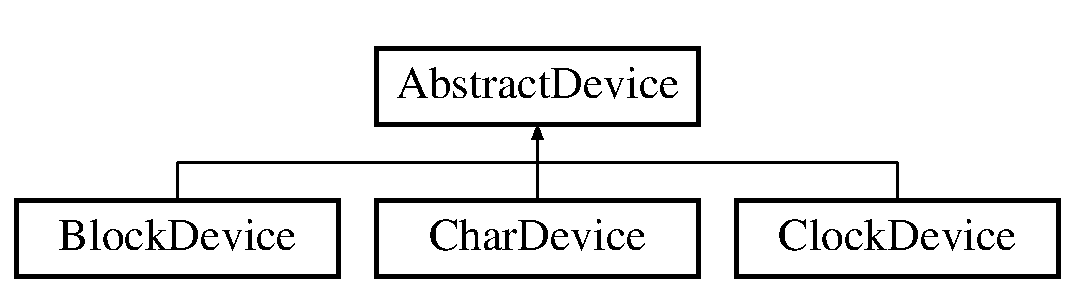
\includegraphics[height=2.000000cm]{db/d0e/classAbstractDevice}
\end{center}
\end{figure}
\subsection*{\-Public \-Member \-Functions}
\begin{DoxyCompactItemize}
\item 
\hypertarget{classAbstractDevice_a393c627235e10b16507161febe32cae0}{virtual void {\bfseries set\-Timer} (int time)=0}\label{db/d0e/classAbstractDevice_a393c627235e10b16507161febe32cae0}

\end{DoxyCompactItemize}


\-The documentation for this class was generated from the following file\-:\begin{DoxyCompactItemize}
\item 
include/devices/abstract\-\_\-device.\-h\end{DoxyCompactItemize}

\hypertarget{classBlockDevice}{\section{\-Block\-Device \-Class \-Reference}
\label{db/d6d/classBlockDevice}\index{\-Block\-Device@{\-Block\-Device}}
}


\-Inheritance diagram for \-Block\-Device\-:\nopagebreak
\begin{figure}[H]
\begin{center}
\leavevmode
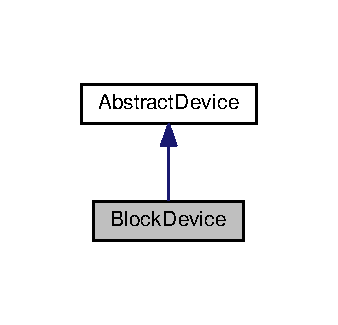
\includegraphics[width=162pt]{d0/d85/classBlockDevice__inherit__graph}
\end{center}
\end{figure}


\-Collaboration diagram for \-Block\-Device\-:\nopagebreak
\begin{figure}[H]
\begin{center}
\leavevmode
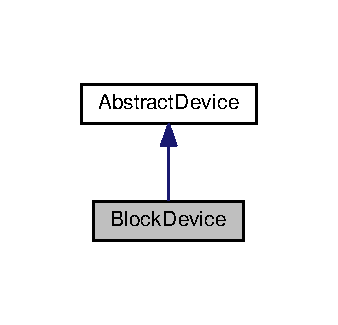
\includegraphics[width=162pt]{d4/df3/classBlockDevice__coll__graph}
\end{center}
\end{figure}
\subsection*{\-Public \-Member \-Functions}
\begin{DoxyCompactItemize}
\item 
\hypertarget{classBlockDevice_a7ff2350ac492e4a73a4b59f9a6bbe629}{void {\bfseries set\-Timer} (int usec)}\label{db/d6d/classBlockDevice_a7ff2350ac492e4a73a4b59f9a6bbe629}

\item 
\hypertarget{classBlockDevice_a442a9657bc83b00f9662138f6f23f925}{void {\bfseries disarm} ()}\label{db/d6d/classBlockDevice_a442a9657bc83b00f9662138f6f23f925}

\end{DoxyCompactItemize}


\-The documentation for this class was generated from the following files\-:\begin{DoxyCompactItemize}
\item 
include/devices/\hyperlink{block__device_8h}{block\-\_\-device.\-h}\item 
src/devices/block\-\_\-device.\-cpp\end{DoxyCompactItemize}

\hypertarget{classcCPU}{\section{c\-C\-P\-U \-Class \-Reference}
\label{d2/dc6/classcCPU}\index{c\-C\-P\-U@{c\-C\-P\-U}}
}


\-A class for emulating a simple cpu.  




{\ttfamily \#include $<$cpu.\-h$>$}

\subsection*{\-Public \-Member \-Functions}
\begin{DoxyCompactItemize}
\item 
void \hyperlink{classcCPU_acd957640be8abb7c0d8a24010ed0e737}{set\-Text} (char $\ast$text)
\begin{DoxyCompactList}\small\item\em \-Set the program text. \end{DoxyCompactList}\item 
void \hyperlink{classcCPU_a176eb207069b99c47ddec6b466d1a92b}{set\-User\-Mode} ()
\begin{DoxyCompactList}\small\item\em \-Set the cpu back into user mode. \end{DoxyCompactList}\item 
unsigned int \hyperlink{classcCPU_ab04938ac939d530e521181db6a52944f}{get\-Set\-P\-C} (unsigned int new\-P\-C)
\begin{DoxyCompactList}\small\item\em \-Get/\-Set the program counter. \end{DoxyCompactList}\item 
int \hyperlink{classcCPU_a2d593a0d3d66e532826db4754d5fc4d2}{get\-Set\-V\-C} (int new\-V\-C)
\begin{DoxyCompactList}\small\item\em \-Get/\-Set the \-V\-C. \end{DoxyCompactList}\item 
uint16\-\_\-t \hyperlink{classcCPU_a0b13774a76c6b04d760b8ff072c37a85}{get\-Set\-P\-S\-W} (uint16\-\_\-t new\-P\-S\-W)
\begin{DoxyCompactList}\small\item\em \-Get/\-Set the \-P\-S\-W. \end{DoxyCompactList}\item 
uint16\-\_\-t \hyperlink{classcCPU_ad485374a709476e2dfb847046d3d5215}{get\-P\-S\-W} ()
\begin{DoxyCompactList}\small\item\em \-Get the \-Program \-Status \-Word. \end{DoxyCompactList}\item 
void \hyperlink{classcCPU_adb6ad793398d28b5615dd1377a619084}{set\-P\-S\-W} (uint16\-\_\-t new\-P\-S\-W)
\begin{DoxyCompactList}\small\item\em \-Set a new value for the \-P\-S\-W. \end{DoxyCompactList}\item 
char $\ast$ \hyperlink{classcCPU_a891d9b77e1818ca247e9d76f4db99415}{get\-Param} (int num)
\begin{DoxyCompactList}\small\item\em \-Get execution parameters from the cpu. \end{DoxyCompactList}\item 
char \hyperlink{classcCPU_a987e1ab511c71dcde48411f5bb16f9d8}{get\-Opcode} ()
\begin{DoxyCompactList}\small\item\em \-Get the current \-Opcode. \end{DoxyCompactList}\item 
void \hyperlink{classcCPU_aee300d68026ba9f13d5434ff82f0372a}{run} ()
\begin{DoxyCompactList}\small\item\em \-Start execution. \end{DoxyCompactList}\end{DoxyCompactItemize}
\subsection*{\-Private \-Member \-Functions}
\begin{DoxyCompactItemize}
\item 
\hypertarget{classcCPU_a62812ecc1a65c296fb4795b24b451f4e}{int {\bfseries tokenize\-Line} ()}\label{d2/dc6/classcCPU_a62812ecc1a65c296fb4795b24b451f4e}

\end{DoxyCompactItemize}
\subsection*{\-Private \-Attributes}
\begin{DoxyCompactItemize}
\item 
\hypertarget{classcCPU_af1d6fd5349bde1621595f6c1422792b4}{bool {\bfseries \-K\-Mode}}\label{d2/dc6/classcCPU_af1d6fd5349bde1621595f6c1422792b4}

\item 
\hypertarget{classcCPU_a982f4af913ec39928e62129200c21e58}{unsigned int {\bfseries \-P\-C}}\label{d2/dc6/classcCPU_a982f4af913ec39928e62129200c21e58}

\item 
\hypertarget{classcCPU_af6d922807d65a8a39722dde518febc52}{unsigned int {\bfseries max\-P\-C}}\label{d2/dc6/classcCPU_af6d922807d65a8a39722dde518febc52}

\item 
\hypertarget{classcCPU_aae9fc88ce939489754ac776b6447607b}{int {\bfseries \-V\-C}}\label{d2/dc6/classcCPU_aae9fc88ce939489754ac776b6447607b}

\item 
\hypertarget{classcCPU_a52457b3189761c2f07c9fb12169dad50}{uint16\-\_\-t \hyperlink{classcCPU_a52457b3189761c2f07c9fb12169dad50}{\-P\-S\-W}}\label{d2/dc6/classcCPU_a52457b3189761c2f07c9fb12169dad50}

\begin{DoxyCompactList}\small\item\em \-Program \-Status \-Word. \end{DoxyCompactList}\item 
\hypertarget{classcCPU_ad50800fe39f7f8d51dc7095e441db94a}{char $\ast$ \hyperlink{classcCPU_ad50800fe39f7f8d51dc7095e441db94a}{exec\-Text}}\label{d2/dc6/classcCPU_ad50800fe39f7f8d51dc7095e441db94a}

\begin{DoxyCompactList}\small\item\em \-Text data for currently executing process. \end{DoxyCompactList}\item 
\hypertarget{classcCPU_a06d3e3497a2636740db81fa00641fd88}{char \hyperlink{classcCPU_a06d3e3497a2636740db81fa00641fd88}{token\-Buffer} \mbox{[}2\mbox{]}\mbox{[}\hyperlink{cpu_8h_a9e34e5196b1f8e4c96f229d062c73fe0}{\-M\-A\-X\-\_\-\-P\-A\-R\-A\-M\-\_\-\-S\-I\-Z\-E}\mbox{]}}\label{d2/dc6/classcCPU_a06d3e3497a2636740db81fa00641fd88}

\begin{DoxyCompactList}\small\item\em \-Holds the tokenized execution parameters. \end{DoxyCompactList}\item 
\hypertarget{classcCPU_a897ce4ac1712c81e8c1a7e13733be8fc}{char \hyperlink{classcCPU_a897ce4ac1712c81e8c1a7e13733be8fc}{\-Opcode}}\label{d2/dc6/classcCPU_a897ce4ac1712c81e8c1a7e13733be8fc}

\begin{DoxyCompactList}\small\item\em \-Holds the current \-Opcode. \end{DoxyCompactList}\end{DoxyCompactItemize}


\subsection{\-Detailed \-Description}
\-This class emulates the internals of a very simple cpu with two main registers, \-P\-C and \-V\-C. \-In addition, it has other state for handling system calls and program exceptions. 

\subsection{\-Member \-Function \-Documentation}
\hypertarget{classcCPU_a987e1ab511c71dcde48411f5bb16f9d8}{\index{c\-C\-P\-U@{c\-C\-P\-U}!get\-Opcode@{get\-Opcode}}
\index{get\-Opcode@{get\-Opcode}!cCPU@{c\-C\-P\-U}}
\subsubsection[{get\-Opcode}]{\setlength{\rightskip}{0pt plus 5cm}char {\bf c\-C\-P\-U\-::get\-Opcode} (
\begin{DoxyParamCaption}
{}
\end{DoxyParamCaption}
)}}\label{d2/dc6/classcCPU_a987e1ab511c71dcde48411f5bb16f9d8}
\-Get the current \-Opcode in the cpu. \-This is used by the kernel to determine which system call as being made. \-Used in conjunciton with \hyperlink{classcCPU_a891d9b77e1818ca247e9d76f4db99415}{c\-C\-P\-U\-::get\-Param} the kernel can process system calls. \hypertarget{classcCPU_a891d9b77e1818ca247e9d76f4db99415}{\index{c\-C\-P\-U@{c\-C\-P\-U}!get\-Param@{get\-Param}}
\index{get\-Param@{get\-Param}!cCPU@{c\-C\-P\-U}}
\subsubsection[{get\-Param}]{\setlength{\rightskip}{0pt plus 5cm}char $\ast$ {\bf c\-C\-P\-U\-::get\-Param} (
\begin{DoxyParamCaption}
\item[{int}]{num}
\end{DoxyParamCaption}
)}}\label{d2/dc6/classcCPU_a891d9b77e1818ca247e9d76f4db99415}
\-Fetch the given execution paramter from the cpu's internal buffer. \-When an instruction is encountered that has parameters associated with it, the cpu tokenizes them and places it in an internal buffer. \-This function is mainly used by the kernel in handling system calls.


\begin{DoxyParams}{\-Parameters}
{\em num} & \-Must be less than \-M\-A\-X\-\_\-\-P\-A\-R\-A\-M\-S (currently 2)\\
\hline
\end{DoxyParams}
\begin{DoxyReturn}{\-Returns}
\-Returns a char$\ast$ which points to a string of at most \-M\-A\-X\-\_\-\-P\-A\-R\-A\-M\-\_\-\-S\-I\-Z\-E -\/ 1 bytes. 
\end{DoxyReturn}
\hypertarget{classcCPU_ad485374a709476e2dfb847046d3d5215}{\index{c\-C\-P\-U@{c\-C\-P\-U}!get\-P\-S\-W@{get\-P\-S\-W}}
\index{get\-P\-S\-W@{get\-P\-S\-W}!cCPU@{c\-C\-P\-U}}
\subsubsection[{get\-P\-S\-W}]{\setlength{\rightskip}{0pt plus 5cm}uint16\-\_\-t {\bf c\-C\-P\-U\-::get\-P\-S\-W} (
\begin{DoxyParamCaption}
{}
\end{DoxyParamCaption}
)}}\label{d2/dc6/classcCPU_ad485374a709476e2dfb847046d3d5215}
\-Returns the program status word which is a unsigned 16-\/bit integer type with flags from \hyperlink{cpu_8h_ade10811b11f1c647313bf0a60797a9f9}{e\-P\-S\-W} set. \-These are used by the kernel to make action decisions. \hypertarget{classcCPU_ab04938ac939d530e521181db6a52944f}{\index{c\-C\-P\-U@{c\-C\-P\-U}!get\-Set\-P\-C@{get\-Set\-P\-C}}
\index{get\-Set\-P\-C@{get\-Set\-P\-C}!cCPU@{c\-C\-P\-U}}
\subsubsection[{get\-Set\-P\-C}]{\setlength{\rightskip}{0pt plus 5cm}unsigned int {\bf c\-C\-P\-U\-::get\-Set\-P\-C} (
\begin{DoxyParamCaption}
\item[{unsigned int}]{new\-P\-C}
\end{DoxyParamCaption}
)}}\label{d2/dc6/classcCPU_ab04938ac939d530e521181db6a52944f}
\-Get the current value for the program counter and then set its value to the given parameter. \-This is useful for swapping out process values. \hypertarget{classcCPU_a0b13774a76c6b04d760b8ff072c37a85}{\index{c\-C\-P\-U@{c\-C\-P\-U}!get\-Set\-P\-S\-W@{get\-Set\-P\-S\-W}}
\index{get\-Set\-P\-S\-W@{get\-Set\-P\-S\-W}!cCPU@{c\-C\-P\-U}}
\subsubsection[{get\-Set\-P\-S\-W}]{\setlength{\rightskip}{0pt plus 5cm}uint16\-\_\-t {\bf c\-C\-P\-U\-::get\-Set\-P\-S\-W} (
\begin{DoxyParamCaption}
\item[{uint16\-\_\-t}]{new\-P\-S\-W}
\end{DoxyParamCaption}
)}}\label{d2/dc6/classcCPU_a0b13774a76c6b04d760b8ff072c37a85}
\-Get the current value for the \-P\-S\-W and set its value to the given parameter. \hypertarget{classcCPU_a2d593a0d3d66e532826db4754d5fc4d2}{\index{c\-C\-P\-U@{c\-C\-P\-U}!get\-Set\-V\-C@{get\-Set\-V\-C}}
\index{get\-Set\-V\-C@{get\-Set\-V\-C}!cCPU@{c\-C\-P\-U}}
\subsubsection[{get\-Set\-V\-C}]{\setlength{\rightskip}{0pt plus 5cm}int {\bf c\-C\-P\-U\-::get\-Set\-V\-C} (
\begin{DoxyParamCaption}
\item[{int}]{new\-V\-C}
\end{DoxyParamCaption}
)}}\label{d2/dc6/classcCPU_a2d593a0d3d66e532826db4754d5fc4d2}
\-Get the current value for \-V\-C and set its value to the given paramter. \-This is useful for swapping out process values. \hypertarget{classcCPU_aee300d68026ba9f13d5434ff82f0372a}{\index{c\-C\-P\-U@{c\-C\-P\-U}!run@{run}}
\index{run@{run}!cCPU@{c\-C\-P\-U}}
\subsubsection[{run}]{\setlength{\rightskip}{0pt plus 5cm}void {\bf c\-C\-P\-U\-::run} (
\begin{DoxyParamCaption}
{}
\end{DoxyParamCaption}
)}}\label{d2/dc6/classcCPU_aee300d68026ba9f13d5434ff82f0372a}
\-Once all appropriate process data is entered by the kernel this function is called to start execution. \-Any time control needs to be returned to the kernel this function will return with the appropriate \-P\-S\-W flags set for the kernel to act on. \hypertarget{classcCPU_adb6ad793398d28b5615dd1377a619084}{\index{c\-C\-P\-U@{c\-C\-P\-U}!set\-P\-S\-W@{set\-P\-S\-W}}
\index{set\-P\-S\-W@{set\-P\-S\-W}!cCPU@{c\-C\-P\-U}}
\subsubsection[{set\-P\-S\-W}]{\setlength{\rightskip}{0pt plus 5cm}void {\bf c\-C\-P\-U\-::set\-P\-S\-W} (
\begin{DoxyParamCaption}
\item[{uint16\-\_\-t}]{new\-P\-S\-W}
\end{DoxyParamCaption}
)}}\label{d2/dc6/classcCPU_adb6ad793398d28b5615dd1377a619084}
\-Used by the kernel to reset the \-P\-S\-W after a system call. \-Any process execution which returns to the kernel but does not terminate the process should reset the \-P\-S\-W so subsequent exceptions/terminations are not lost by stray \-P\-S\-W values. \hypertarget{classcCPU_acd957640be8abb7c0d8a24010ed0e737}{\index{c\-C\-P\-U@{c\-C\-P\-U}!set\-Text@{set\-Text}}
\index{set\-Text@{set\-Text}!cCPU@{c\-C\-P\-U}}
\subsubsection[{set\-Text}]{\setlength{\rightskip}{0pt plus 5cm}void {\bf c\-C\-P\-U\-::set\-Text} (
\begin{DoxyParamCaption}
\item[{char $\ast$}]{text}
\end{DoxyParamCaption}
)}}\label{d2/dc6/classcCPU_acd957640be8abb7c0d8a24010ed0e737}
\-Point the cpu to the text data for the running process. \-This text is indexed using the program counter (\-P\-C).


\begin{DoxyParams}{\-Parameters}
{\em text} & \-Program text pointer. assert( text != \-N\-U\-L\-L) \\
\hline
\end{DoxyParams}
\hypertarget{classcCPU_a176eb207069b99c47ddec6b466d1a92b}{\index{c\-C\-P\-U@{c\-C\-P\-U}!set\-User\-Mode@{set\-User\-Mode}}
\index{set\-User\-Mode@{set\-User\-Mode}!cCPU@{c\-C\-P\-U}}
\subsubsection[{set\-User\-Mode}]{\setlength{\rightskip}{0pt plus 5cm}void {\bf c\-C\-P\-U\-::set\-User\-Mode} (
\begin{DoxyParamCaption}
{}
\end{DoxyParamCaption}
)}}\label{d2/dc6/classcCPU_a176eb207069b99c47ddec6b466d1a92b}
\-This is used by the kernel after the kernel has finished servicing a process' kernel mode request (syscall). 

\-The documentation for this class was generated from the following files\-:\begin{DoxyCompactItemize}
\item 
include/\hyperlink{cpu_8h}{cpu.\-h}\item 
src/cpu.\-cpp\end{DoxyCompactItemize}

\hypertarget{classcFCFS}{\section{c\-F\-C\-F\-S \-Class \-Reference}
\label{d6/dc3/classcFCFS}\index{c\-F\-C\-F\-S@{c\-F\-C\-F\-S}}
}
\-Inheritance diagram for c\-F\-C\-F\-S\-:\begin{figure}[H]
\begin{center}
\leavevmode
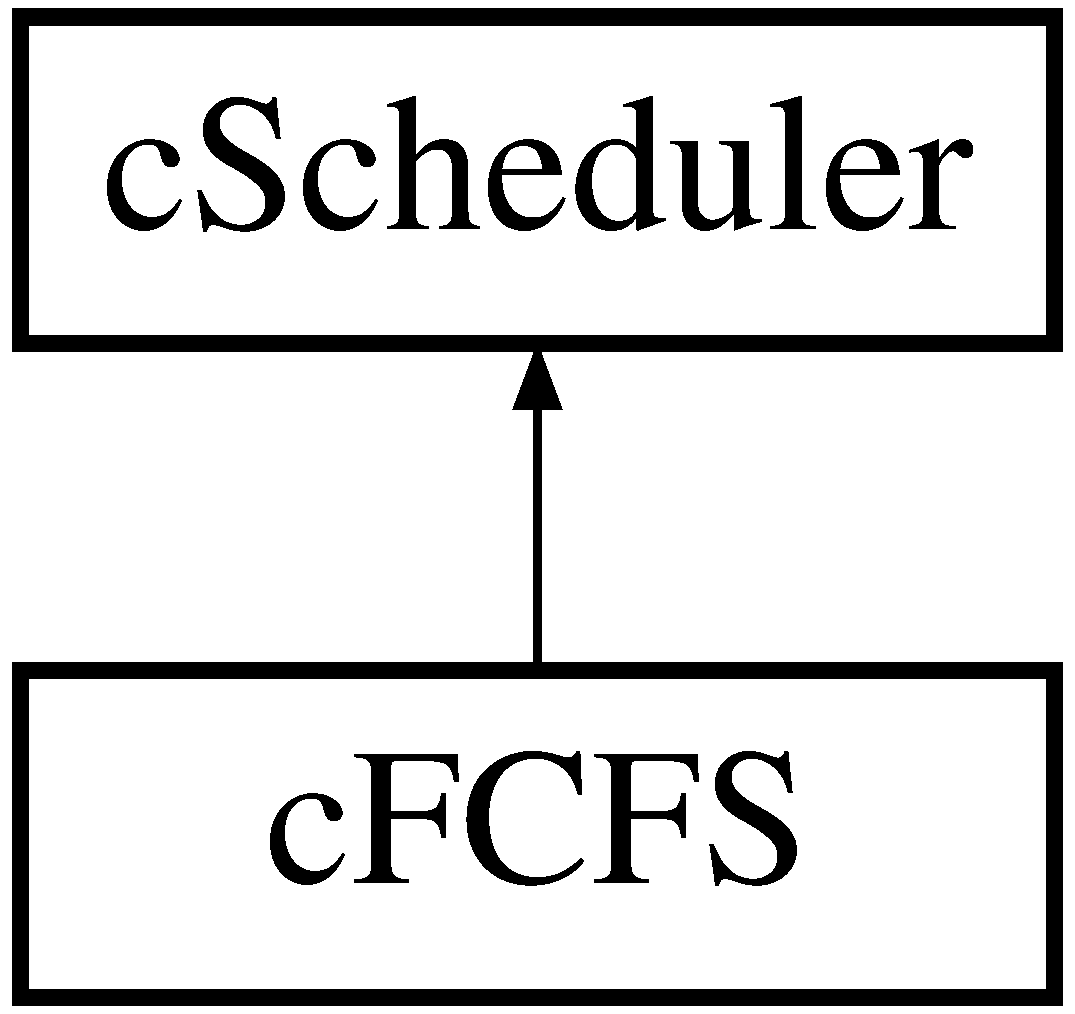
\includegraphics[height=2.000000cm]{d6/dc3/classcFCFS}
\end{center}
\end{figure}
\subsection*{\-Public \-Member \-Functions}
\begin{DoxyCompactItemize}
\item 
\hypertarget{classcFCFS_aff34f18c6f4c3f38029d904cd2ec55de}{void {\bfseries init\-Proc\-Schedule\-Info} (\hyperlink{structProcessInfo}{\-Process\-Info} $\ast$)}\label{d6/dc3/classcFCFS_aff34f18c6f4c3f38029d904cd2ec55de}

\item 
\hypertarget{classcFCFS_a1b8ee3a759a31032ec7c1cd7b15ed5df}{void {\bfseries set\-Blocked} (\hyperlink{structProcessInfo}{\-Process\-Info} $\ast$)}\label{d6/dc3/classcFCFS_a1b8ee3a759a31032ec7c1cd7b15ed5df}

\item 
\hypertarget{classcFCFS_ab0c26f757ad8dda985d4f0295f05c781}{void {\bfseries set\-Runnable} (\hyperlink{structProcessInfo}{\-Process\-Info} $\ast$)}\label{d6/dc3/classcFCFS_ab0c26f757ad8dda985d4f0295f05c781}

\item 
\hypertarget{classcFCFS_aeeac757885108ae510b728600ebba248}{void {\bfseries remove\-Process} (\hyperlink{structProcessInfo}{\-Process\-Info} $\ast$)}\label{d6/dc3/classcFCFS_aeeac757885108ae510b728600ebba248}

\item 
\hypertarget{classcFCFS_a3e8a539b117b0eebc991e49dba9638ca}{virtual unsigned int {\bfseries get\-Next\-To\-Run} ()}\label{d6/dc3/classcFCFS_a3e8a539b117b0eebc991e49dba9638ca}

\end{DoxyCompactItemize}


\-The documentation for this class was generated from the following files\-:\begin{DoxyCompactItemize}
\item 
include/scheduler/fcfs.\-h\item 
src/scheduler/fcfs.\-cpp\end{DoxyCompactItemize}

\hypertarget{classCharDevice}{\section{\-Char\-Device \-Class \-Reference}
\label{d8/d4f/classCharDevice}\index{\-Char\-Device@{\-Char\-Device}}
}
\-Inheritance diagram for \-Char\-Device\-:\begin{figure}[H]
\begin{center}
\leavevmode
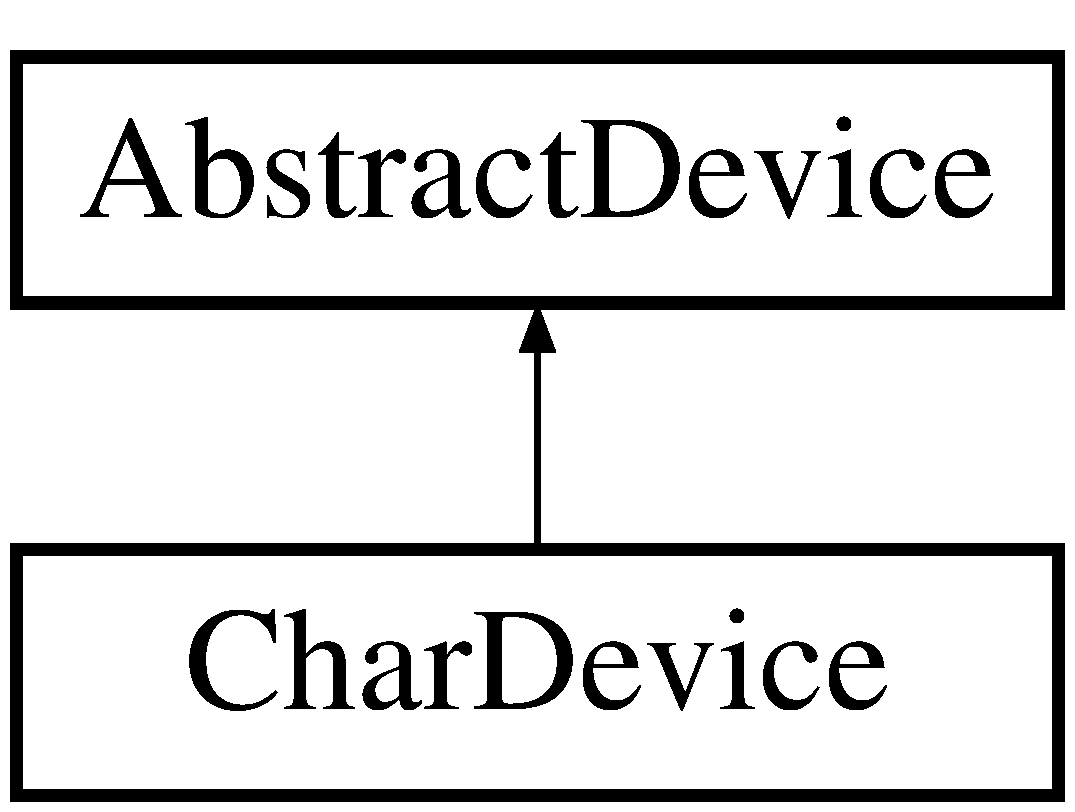
\includegraphics[height=2.000000cm]{d8/d4f/classCharDevice}
\end{center}
\end{figure}
\subsection*{\-Public \-Member \-Functions}
\begin{DoxyCompactItemize}
\item 
\hypertarget{classCharDevice_a8689c0a03b971367322a9dd25bcfb7db}{void {\bfseries set\-Timer} (int usec)}\label{d8/d4f/classCharDevice_a8689c0a03b971367322a9dd25bcfb7db}

\end{DoxyCompactItemize}


\-The documentation for this class was generated from the following files\-:\begin{DoxyCompactItemize}
\item 
include/devices/char\-\_\-device.\-h\item 
src/devices/char\-\_\-device.\-cpp\end{DoxyCompactItemize}

\hypertarget{classcIDManager}{\section{c\-I\-D\-Manager \-Class \-Reference}
\label{de/dd4/classcIDManager}\index{c\-I\-D\-Manager@{c\-I\-D\-Manager}}
}


\-Collaboration diagram for c\-I\-D\-Manager\-:\nopagebreak
\begin{figure}[H]
\begin{center}
\leavevmode
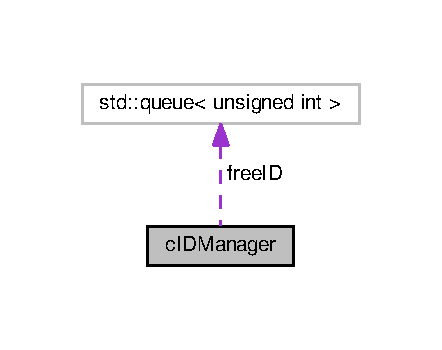
\includegraphics[width=212pt]{db/d8e/classcIDManager__coll__graph}
\end{center}
\end{figure}
\subsection*{\-Public \-Member \-Functions}
\begin{DoxyCompactItemize}
\item 
\hyperlink{classcIDManager_a59021595aaf85ebc151c207a8a04f101}{c\-I\-D\-Manager} (unsigned int start\-I\-D=0)
\begin{DoxyCompactList}\small\item\em \-Creates a new \-I\-D \-Manager object. \end{DoxyCompactList}\item 
unsigned int \hyperlink{classcIDManager_a45420147e785cc219743e9aa2c336501}{get\-I\-D} ()
\begin{DoxyCompactList}\small\item\em \-Reserves a unique \-I\-D. \end{DoxyCompactList}\item 
void \hyperlink{classcIDManager_a6671d898740f88cf40860b0b9e119b02}{return\-I\-D} (unsigned int id)
\begin{DoxyCompactList}\small\item\em \-Returns an \-I\-D to the manager. \end{DoxyCompactList}\end{DoxyCompactItemize}
\subsection*{\-Private \-Attributes}
\begin{DoxyCompactItemize}
\item 
\hypertarget{classcIDManager_a0bed8666fa886f86428e7ac059bc5de0}{queue$<$ unsigned int $>$ {\bfseries free\-I\-D}}\label{de/dd4/classcIDManager_a0bed8666fa886f86428e7ac059bc5de0}

\item 
\hypertarget{classcIDManager_a951329fb713c227a88b8db71e0f09e9c}{unsigned int {\bfseries current\-I\-D}}\label{de/dd4/classcIDManager_a951329fb713c227a88b8db71e0f09e9c}

\item 
\hypertarget{classcIDManager_a8e7c466b5b71bf46a203d3c92533daa0}{bool {\bfseries consume\-Queue}}\label{de/dd4/classcIDManager_a8e7c466b5b71bf46a203d3c92533daa0}

\end{DoxyCompactItemize}


\subsection{\-Constructor \& \-Destructor \-Documentation}
\hypertarget{classcIDManager_a59021595aaf85ebc151c207a8a04f101}{\index{c\-I\-D\-Manager@{c\-I\-D\-Manager}!c\-I\-D\-Manager@{c\-I\-D\-Manager}}
\index{c\-I\-D\-Manager@{c\-I\-D\-Manager}!cIDManager@{c\-I\-D\-Manager}}
\subsubsection[{c\-I\-D\-Manager}]{\setlength{\rightskip}{0pt plus 5cm}{\bf c\-I\-D\-Manager\-::c\-I\-D\-Manager} (
\begin{DoxyParamCaption}
\item[{unsigned int}]{start\-I\-D = {\ttfamily 0}}
\end{DoxyParamCaption}
)}}\label{de/dd4/classcIDManager_a59021595aaf85ebc151c207a8a04f101}
\-Default start \-I\-D is 0. 

\subsection{\-Member \-Function \-Documentation}
\hypertarget{classcIDManager_a45420147e785cc219743e9aa2c336501}{\index{c\-I\-D\-Manager@{c\-I\-D\-Manager}!get\-I\-D@{get\-I\-D}}
\index{get\-I\-D@{get\-I\-D}!cIDManager@{c\-I\-D\-Manager}}
\subsubsection[{get\-I\-D}]{\setlength{\rightskip}{0pt plus 5cm}unsigned int {\bf c\-I\-D\-Manager\-::get\-I\-D} (
\begin{DoxyParamCaption}
{}
\end{DoxyParamCaption}
)}}\label{de/dd4/classcIDManager_a45420147e785cc219743e9aa2c336501}
\-Unique is in the sense that no one else is currently using it but it may have been used previously. are distributed in increasing order until \-U\-I\-N\-T\-\_\-\-M\-A\-X is reached. \-After this is reached, \-I\-Ds are given from the queue of returned \-I\-Ds. \-If this queue is empty then an exception is thrown. \hypertarget{classcIDManager_a6671d898740f88cf40860b0b9e119b02}{\index{c\-I\-D\-Manager@{c\-I\-D\-Manager}!return\-I\-D@{return\-I\-D}}
\index{return\-I\-D@{return\-I\-D}!cIDManager@{c\-I\-D\-Manager}}
\subsubsection[{return\-I\-D}]{\setlength{\rightskip}{0pt plus 5cm}void {\bf c\-I\-D\-Manager\-::return\-I\-D} (
\begin{DoxyParamCaption}
\item[{unsigned int}]{id}
\end{DoxyParamCaption}
)}}\label{de/dd4/classcIDManager_a6671d898740f88cf40860b0b9e119b02}
\-If the \-I\-D is not equal to the one last given then it is added to a 'free queue'. \-If it is equal to the last one reserved then the \-I\-D counter is simply decremented \-If this last case happens, it causes \hyperlink{classcIDManager_a45420147e785cc219743e9aa2c336501}{c\-I\-D\-Manager\-::get\-I\-D} to stop consuming from the queue and return this newly availabe \-I\-D. 

\-The documentation for this class was generated from the following files\-:\begin{DoxyCompactItemize}
\item 
include/utility/id.\-h\item 
src/utility/id.\-cpp\end{DoxyCompactItemize}

\hypertarget{classcKernel}{\section{c\-Kernel \-Class \-Reference}
\label{db/da5/classcKernel}\index{c\-Kernel@{c\-Kernel}}
}


\-Collaboration diagram for c\-Kernel\-:\nopagebreak
\begin{figure}[H]
\begin{center}
\leavevmode
\includegraphics[width=350pt]{d4/d6f/classcKernel__coll__graph}
\end{center}
\end{figure}
\subsection*{\-Public \-Member \-Functions}
\begin{DoxyCompactItemize}
\item 
\hyperlink{classcKernel_a64d105a595a4d14a47bb65426b331159}{c\-Kernel} ()
\begin{DoxyCompactList}\small\item\em \-Default \hyperlink{classcKernel}{c\-Kernel} constructor. \end{DoxyCompactList}\item 
void \hyperlink{classcKernel_a0ce9a2721bb1ea4d7f999198634f702d}{boot} ()
\begin{DoxyCompactList}\small\item\em \-Start the '\-O\-S' \-Kernel. \end{DoxyCompactList}\item 
void \hyperlink{classcKernel_a5440eace2647ffd5279de55600947b84}{init\-Process} (const char $\ast$filename, pid\-Type parent, int priority=\hyperlink{kernel_8h_a0756f011ef667460d583017366823244}{\-D\-E\-F\-A\-U\-L\-T\-\_\-\-P\-R\-I\-O\-R\-I\-T\-Y})
\begin{DoxyCompactList}\small\item\em \-Initialize a \-Process. \end{DoxyCompactList}\item 
void \hyperlink{classcKernel_a1e7cb5c6d9e6140e197f9b18dc8bd1b1}{cleanup\-Process} (pid\-Type pid)
\begin{DoxyCompactList}\small\item\em \-Cleans up a terminated process. \end{DoxyCompactList}\end{DoxyCompactItemize}
\subsection*{\-Private \-Member \-Functions}
\begin{DoxyCompactItemize}
\item 
void \hyperlink{classcKernel_a1b8e06f240c1bb7d0c4d0d30bcc55e18}{swap\-Processes} (\hyperlink{structProcessInfo}{\-Process\-Info} $\ast$proc, bool switch\-Mode=true)
\begin{DoxyCompactList}\small\item\em \-Swap a process on the cpu. \end{DoxyCompactList}\item 
\hypertarget{classcKernel_abcc0464e62a5fb82ddf4a3f8ba5ec461}{void {\bfseries cleanup\-Process} (\hyperlink{structProcessInfo}{\-Process\-Info} $\ast$)}\label{db/da5/classcKernel_abcc0464e62a5fb82ddf4a3f8ba5ec461}

\item 
void \hyperlink{classcKernel_a60ccaffeee3cfcfdfb4aa7b9e33b19f4}{sig\-Handler} (int signum, siginfo\-\_\-t $\ast$info)
\begin{DoxyCompactList}\small\item\em \-Handler for all signals. \end{DoxyCompactList}\end{DoxyCompactItemize}
\subsection*{\-Static \-Private \-Member \-Functions}
\begin{DoxyCompactItemize}
\item 
\hypertarget{classcKernel_a571bb344ba50970d9c4a1cb5b500bbcd}{static void {\bfseries sig\-\_\-catch} (int signum, siginfo\-\_\-t $\ast$info, void $\ast$context)}\label{db/da5/classcKernel_a571bb344ba50970d9c4a1cb5b500bbcd}

\end{DoxyCompactItemize}
\subsection*{\-Private \-Attributes}
\begin{DoxyCompactItemize}
\item 
\hypertarget{classcKernel_a7b4ac330752179e72a5e440d30c64e91}{\-F\-I\-L\-E $\ast$ {\bfseries trace\-Stream}}\label{db/da5/classcKernel_a7b4ac330752179e72a5e440d30c64e91}

\item 
\hypertarget{classcKernel_a1fb233fa1c51650ccf2c872d856329ff}{\hyperlink{classcCPU}{c\-C\-P\-U} {\bfseries cpu}}\label{db/da5/classcKernel_a1fb233fa1c51650ccf2c872d856329ff}

\item 
\hypertarget{classcKernel_a1de4acdb706016573445b3c497e3b508}{int {\bfseries clock\-Tick}}\label{db/da5/classcKernel_a1de4acdb706016573445b3c497e3b508}

\item 
\hypertarget{classcKernel_a61c0f8a08a605a92c564056bb34f6957}{pthread\-\_\-mutex\-\_\-t {\bfseries int\-Lock}}\label{db/da5/classcKernel_a61c0f8a08a605a92c564056bb34f6957}

\item 
\hypertarget{classcKernel_a81cad8017ccbb1768ee0aa9aa2fcf056}{pthread\-\_\-cond\-\_\-t {\bfseries int\-Cond}}\label{db/da5/classcKernel_a81cad8017ccbb1768ee0aa9aa2fcf056}

\item 
\hypertarget{classcKernel_a2d05550b96d1a4c4b02d523574fa94b3}{\hyperlink{classBlockDevice}{\-Block\-Device} {\bfseries b\-Device}}\label{db/da5/classcKernel_a2d05550b96d1a4c4b02d523574fa94b3}

\item 
\hypertarget{classcKernel_abe168524c497a731b708eeeffa810a4b}{\hyperlink{classCharDevice}{\-Char\-Device} {\bfseries c\-Device}}\label{db/da5/classcKernel_abe168524c497a731b708eeeffa810a4b}

\item 
\hypertarget{classcKernel_a1e82363115819c11c74ac261d82d11b5}{\hyperlink{classClockDevice}{\-Clock\-Device} {\bfseries clock\-Interrupt}}\label{db/da5/classcKernel_a1e82363115819c11c74ac261d82d11b5}

\item 
\hypertarget{classcKernel_a6e33ce858b1839bbeb6503515bf11475}{\hyperlink{structProcessInfo}{\-Process\-Info} $\ast$ \hyperlink{classcKernel_a6e33ce858b1839bbeb6503515bf11475}{running\-Proc}}\label{db/da5/classcKernel_a6e33ce858b1839bbeb6503515bf11475}

\begin{DoxyCompactList}\small\item\em \hyperlink{structProcessInfo}{\-Process\-Info} \end{DoxyCompactList}\item 
\hypertarget{classcKernel_a03d2c6943661797e86c030864890183e}{\hyperlink{classcIDManager}{c\-I\-D\-Manager} {\bfseries id\-Generator}}\label{db/da5/classcKernel_a03d2c6943661797e86c030864890183e}

\item 
\hypertarget{classcKernel_a739c2652aee254fc800e8fe05452db8c}{\hyperlink{classcFCFS}{scheduler\-Type} {\bfseries scheduler}}\label{db/da5/classcKernel_a739c2652aee254fc800e8fe05452db8c}

\end{DoxyCompactItemize}
\subsection*{\-Static \-Private \-Attributes}
\begin{DoxyCompactItemize}
\item 
\hypertarget{classcKernel_ae757ff0479ba7ce5154aff58f493cfa9}{static \hyperlink{classcKernel}{c\-Kernel} $\ast$ {\bfseries kernel\-\_\-instance}}\label{db/da5/classcKernel_ae757ff0479ba7ce5154aff58f493cfa9}

\end{DoxyCompactItemize}


\subsection{\-Constructor \& \-Destructor \-Documentation}
\hypertarget{classcKernel_a64d105a595a4d14a47bb65426b331159}{\index{c\-Kernel@{c\-Kernel}!c\-Kernel@{c\-Kernel}}
\index{c\-Kernel@{c\-Kernel}!cKernel@{c\-Kernel}}
\subsubsection[{c\-Kernel}]{\setlength{\rightskip}{0pt plus 5cm}{\bf c\-Kernel\-::c\-Kernel} (
\begin{DoxyParamCaption}
{}
\end{DoxyParamCaption}
)}}\label{db/da5/classcKernel_a64d105a595a4d14a47bb65426b331159}
\-The default constructor initializes all internal datastructures and loads the initial program (default\-: 'main.\-trace') but does not run it. 

\subsection{\-Member \-Function \-Documentation}
\hypertarget{classcKernel_a0ce9a2721bb1ea4d7f999198634f702d}{\index{c\-Kernel@{c\-Kernel}!boot@{boot}}
\index{boot@{boot}!cKernel@{c\-Kernel}}
\subsubsection[{boot}]{\setlength{\rightskip}{0pt plus 5cm}void {\bf c\-Kernel\-::boot} (
\begin{DoxyParamCaption}
{}
\end{DoxyParamCaption}
)}}\label{db/da5/classcKernel_a0ce9a2721bb1ea4d7f999198634f702d}
\-Starts the main kernel loop. \-The initial program is loaded and execution follows from there.


\begin{DoxyExceptions}{\-Exceptions}
{\em \hyperlink{structkernelError}{kernel\-Error}} & \\
\hline
\end{DoxyExceptions}
\hypertarget{classcKernel_a1e7cb5c6d9e6140e197f9b18dc8bd1b1}{\index{c\-Kernel@{c\-Kernel}!cleanup\-Process@{cleanup\-Process}}
\index{cleanup\-Process@{cleanup\-Process}!cKernel@{c\-Kernel}}
\subsubsection[{cleanup\-Process}]{\setlength{\rightskip}{0pt plus 5cm}void c\-Kernel\-::cleanup\-Process (
\begin{DoxyParamCaption}
\item[{pid\-Type}]{pid}
\end{DoxyParamCaption}
)}}\label{db/da5/classcKernel_a1e7cb5c6d9e6140e197f9b18dc8bd1b1}
\-Cleans up any memory and kernel entries associated with the terminated process. \-Also removes the process from the scheduler. \hypertarget{classcKernel_a5440eace2647ffd5279de55600947b84}{\index{c\-Kernel@{c\-Kernel}!init\-Process@{init\-Process}}
\index{init\-Process@{init\-Process}!cKernel@{c\-Kernel}}
\subsubsection[{init\-Process}]{\setlength{\rightskip}{0pt plus 5cm}void {\bf c\-Kernel\-::init\-Process} (
\begin{DoxyParamCaption}
\item[{const char $\ast$}]{filename, }
\item[{pid\-Type}]{parent, }
\item[{int}]{priority = {\ttfamily {\bf \-D\-E\-F\-A\-U\-L\-T\-\_\-\-P\-R\-I\-O\-R\-I\-T\-Y}}}
\end{DoxyParamCaption}
)}}\label{db/da5/classcKernel_a5440eace2647ffd5279de55600947b84}
\-Initializes a process by loading program file contents, setting default process values and adding it in a ready state to the scheduler. \hypertarget{classcKernel_a60ccaffeee3cfcfdfb4aa7b9e33b19f4}{\index{c\-Kernel@{c\-Kernel}!sig\-Handler@{sig\-Handler}}
\index{sig\-Handler@{sig\-Handler}!cKernel@{c\-Kernel}}
\subsubsection[{sig\-Handler}]{\setlength{\rightskip}{0pt plus 5cm}void {\bf c\-Kernel\-::sig\-Handler} (
\begin{DoxyParamCaption}
\item[{int}]{signum, }
\item[{siginfo\-\_\-t $\ast$}]{info}
\end{DoxyParamCaption}
)\hspace{0.3cm}{\ttfamily  \mbox{[}private\mbox{]}}}}\label{db/da5/classcKernel_a60ccaffeee3cfcfdfb4aa7b9e33b19f4}
\-Each device uses a timer from \-S\-I\-G\-R\-T\-M\-I\-N -\/$>$ \-S\-I\-G\-R\-T\-M\-A\-X. \-Because these are not required to be compile time constants, a switch statement cannot be used. \-When a signal is received by the kernel, careful consideration must be made to the current state. \-Below is each signal and how it is handled\-: \hypertarget{classcKernel_a1b8e06f240c1bb7d0c4d0d30bcc55e18}{\index{c\-Kernel@{c\-Kernel}!swap\-Processes@{swap\-Processes}}
\index{swap\-Processes@{swap\-Processes}!cKernel@{c\-Kernel}}
\subsubsection[{swap\-Processes}]{\setlength{\rightskip}{0pt plus 5cm}void {\bf c\-Kernel\-::swap\-Processes} (
\begin{DoxyParamCaption}
\item[{{\bf \-Process\-Info} $\ast$}]{proc, }
\item[{bool}]{switch\-Mode = {\ttfamily true}}
\end{DoxyParamCaption}
)\hspace{0.3cm}{\ttfamily  \mbox{[}private\mbox{]}}}}\label{db/da5/classcKernel_a1b8e06f240c1bb7d0c4d0d30bcc55e18}
\-Takes the process in its parameter and swaps it with the one currently running in the cpu. 

\-The documentation for this class was generated from the following files\-:\begin{DoxyCompactItemize}
\item 
include/\hyperlink{kernel_8h}{kernel.\-h}\item 
src/kernel.\-cpp\end{DoxyCompactItemize}

\hypertarget{classClockDevice}{\section{\-Clock\-Device \-Class \-Reference}
\label{dc/d14/classClockDevice}\index{\-Clock\-Device@{\-Clock\-Device}}
}


\-Device for generating repeated clock interrupts.  




{\ttfamily \#include $<$clock\-\_\-device.\-h$>$}



\-Inheritance diagram for \-Clock\-Device\-:\nopagebreak
\begin{figure}[H]
\begin{center}
\leavevmode
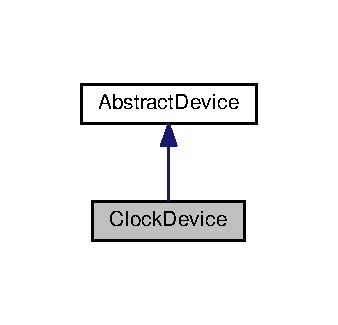
\includegraphics[width=162pt]{de/da0/classClockDevice__inherit__graph}
\end{center}
\end{figure}


\-Collaboration diagram for \-Clock\-Device\-:\nopagebreak
\begin{figure}[H]
\begin{center}
\leavevmode
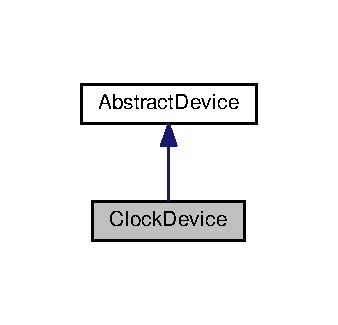
\includegraphics[width=162pt]{d5/d1e/classClockDevice__coll__graph}
\end{center}
\end{figure}
\subsection*{\-Public \-Member \-Functions}
\begin{DoxyCompactItemize}
\item 
void \hyperlink{classClockDevice_a780eebde86fb6a6400894128ac37fa37}{set\-Timer} (int usec)
\begin{DoxyCompactList}\small\item\em \-Set the timer to go off. \end{DoxyCompactList}\item 
void \hyperlink{classClockDevice_a0a0c99ba88b7d0cfaccd09d774c726fe}{disarm} ()
\begin{DoxyCompactList}\small\item\em \-Disarm the timer. \end{DoxyCompactList}\item 
int \hyperlink{classClockDevice_a6dd7b50cf793e37514890eff3e7adf95}{get\-Time} ()
\begin{DoxyCompactList}\small\item\em \-Get how much time is remaining. \end{DoxyCompactList}\end{DoxyCompactItemize}


\subsection{\-Member \-Function \-Documentation}
\hypertarget{classClockDevice_a0a0c99ba88b7d0cfaccd09d774c726fe}{\index{\-Clock\-Device@{\-Clock\-Device}!disarm@{disarm}}
\index{disarm@{disarm}!ClockDevice@{\-Clock\-Device}}
\subsubsection[{disarm}]{\setlength{\rightskip}{0pt plus 5cm}void {\bf \-Clock\-Device\-::disarm} (
\begin{DoxyParamCaption}
{}
\end{DoxyParamCaption}
)\hspace{0.3cm}{\ttfamily  \mbox{[}virtual\mbox{]}}}}\label{dc/d14/classClockDevice_a0a0c99ba88b7d0cfaccd09d774c726fe}
\-Tries to disarm the timer.


\begin{DoxyExceptions}{\-Exceptions}
{\em std\-::string} & error message \\
\hline
\end{DoxyExceptions}


\-Implements \hyperlink{classAbstractDevice_a79059fee864bb0cca04e57e5f5a84401}{\-Abstract\-Device}.

\hypertarget{classClockDevice_a6dd7b50cf793e37514890eff3e7adf95}{\index{\-Clock\-Device@{\-Clock\-Device}!get\-Time@{get\-Time}}
\index{get\-Time@{get\-Time}!ClockDevice@{\-Clock\-Device}}
\subsubsection[{get\-Time}]{\setlength{\rightskip}{0pt plus 5cm}int {\bf \-Clock\-Device\-::get\-Time} (
\begin{DoxyParamCaption}
{}
\end{DoxyParamCaption}
)}}\label{dc/d14/classClockDevice_a6dd7b50cf793e37514890eff3e7adf95}
\-Returns the remaining time until a signal is produced.

\begin{DoxyReturn}{\-Returns}
int \-Time left in microseconds 
\end{DoxyReturn}
\hypertarget{classClockDevice_a780eebde86fb6a6400894128ac37fa37}{\index{\-Clock\-Device@{\-Clock\-Device}!set\-Timer@{set\-Timer}}
\index{set\-Timer@{set\-Timer}!ClockDevice@{\-Clock\-Device}}
\subsubsection[{set\-Timer}]{\setlength{\rightskip}{0pt plus 5cm}void {\bf \-Clock\-Device\-::set\-Timer} (
\begin{DoxyParamCaption}
\item[{int}]{usec}
\end{DoxyParamCaption}
)\hspace{0.3cm}{\ttfamily  \mbox{[}virtual\mbox{]}}}}\label{dc/d14/classClockDevice_a780eebde86fb6a6400894128ac37fa37}
\-Sets timer to send signal \hyperlink{clock__device_8h_af6318deadd0687fb8ffb5437eaa1870d}{\-C\-L\-O\-C\-K\-S\-I\-G} in usec microseconds.


\begin{DoxyParams}{\-Parameters}
{\em usec} & \-Time in microseconds.\\
\hline
\end{DoxyParams}

\begin{DoxyExceptions}{\-Exceptions}
{\em std\-::string} & error message \\
\hline
\end{DoxyExceptions}


\-Implements \hyperlink{classAbstractDevice_adbf2b1dbd7d51896697fce8ae924f286}{\-Abstract\-Device}.



\-Referenced by c\-Kernel\-::boot().



\-The documentation for this class was generated from the following files\-:\begin{DoxyCompactItemize}
\item 
include/devices/\hyperlink{clock__device_8h}{clock\-\_\-device.\-h}\item 
src/devices/clock\-\_\-device.\-cpp\end{DoxyCompactItemize}

\hypertarget{classcRoundRobin}{\section{c\-Round\-Robin \-Class \-Reference}
\label{dc/dcc/classcRoundRobin}\index{c\-Round\-Robin@{c\-Round\-Robin}}
}


\-Round \-Robin \-Scheduler.  




{\ttfamily \#include $<$round\-\_\-robin.\-h$>$}



\-Inheritance diagram for c\-Round\-Robin\-:\nopagebreak
\begin{figure}[H]
\begin{center}
\leavevmode
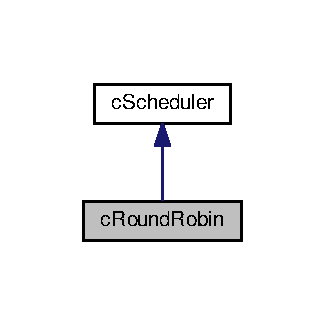
\includegraphics[width=156pt]{d7/de9/classcRoundRobin__inherit__graph}
\end{center}
\end{figure}


\-Collaboration diagram for c\-Round\-Robin\-:\nopagebreak
\begin{figure}[H]
\begin{center}
\leavevmode
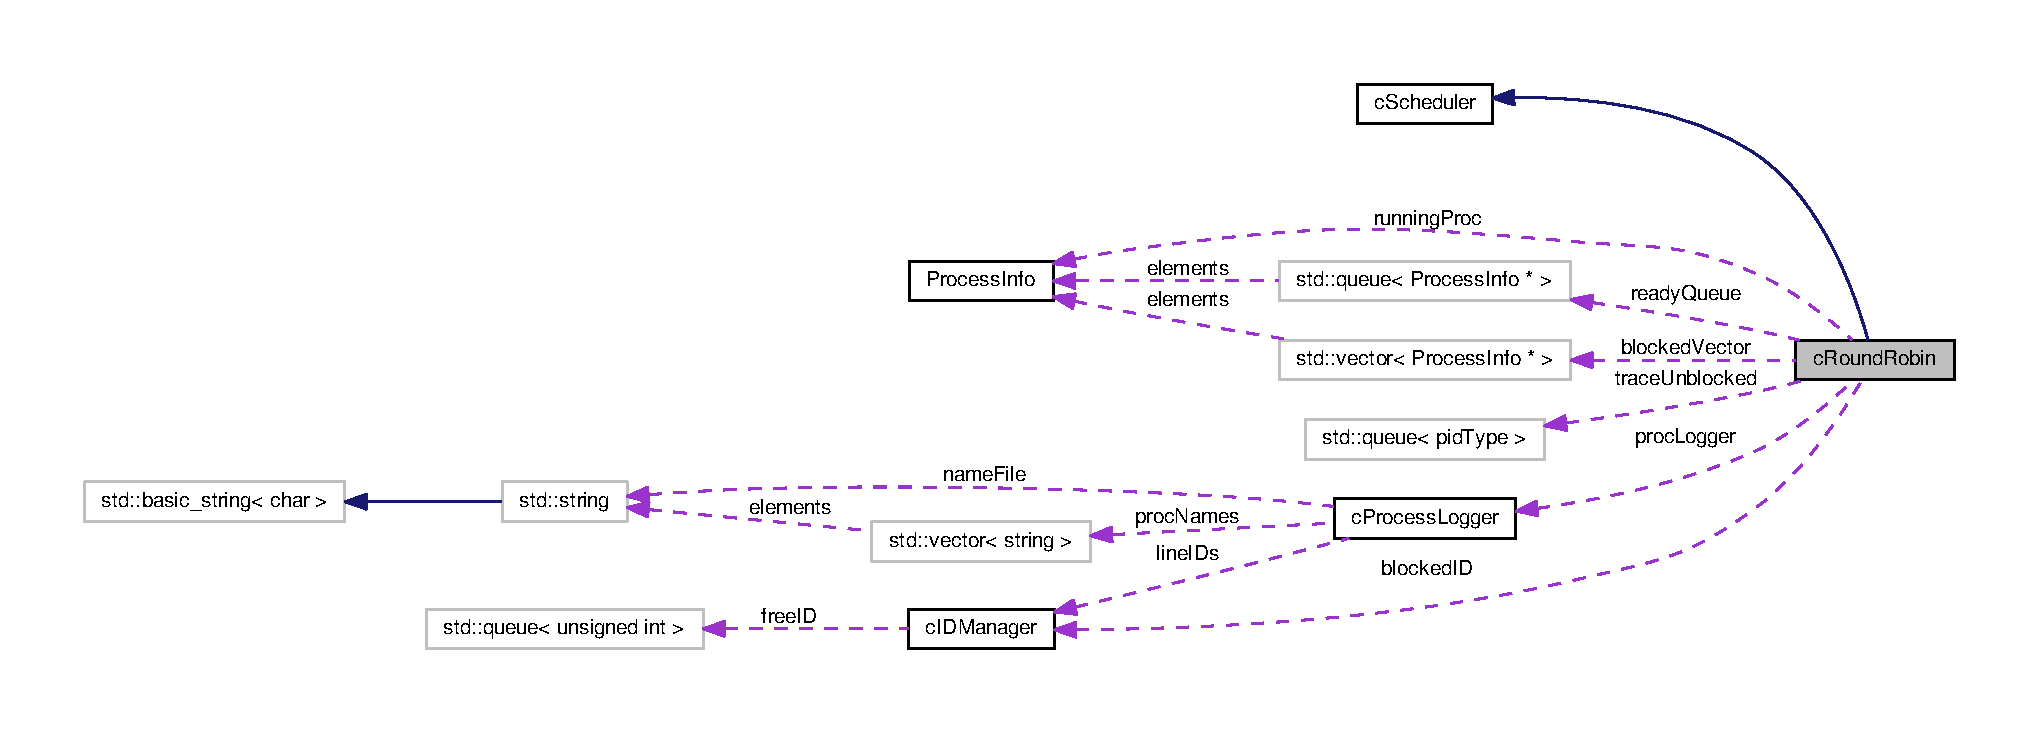
\includegraphics[width=350pt]{de/d42/classcRoundRobin__coll__graph}
\end{center}
\end{figure}
\subsection*{\-Public \-Member \-Functions}
\begin{DoxyCompactItemize}
\item 
\hypertarget{classcRoundRobin_aadb221df9b12f61c3151996ea5c09741}{void \hyperlink{classcRoundRobin_aadb221df9b12f61c3151996ea5c09741}{init\-Proc\-Schedule\-Info} (\hyperlink{structProcessInfo}{\-Process\-Info} $\ast$)}\label{dc/dcc/classcRoundRobin_aadb221df9b12f61c3151996ea5c09741}

\begin{DoxyCompactList}\small\item\em \-Initializes a new \hyperlink{structroundRobinInfo}{round\-Robin\-Info} struct. \end{DoxyCompactList}\item 
\hypertarget{classcRoundRobin_a3571d05a8daebccb758d63b8327f8a22}{void \hyperlink{classcRoundRobin_a3571d05a8daebccb758d63b8327f8a22}{add\-Process} (\hyperlink{structProcessInfo}{\-Process\-Info} $\ast$)}\label{dc/dcc/classcRoundRobin_a3571d05a8daebccb758d63b8327f8a22}

\begin{DoxyCompactList}\small\item\em \-Adds a process to the back of the ready\-Queue. \end{DoxyCompactList}\item 
void \hyperlink{classcRoundRobin_a13609de0f36c81a780072f9c0730f963}{set\-Blocked} (\hyperlink{structProcessInfo}{\-Process\-Info} $\ast$)
\begin{DoxyCompactList}\small\item\em \-Adds a process to the blocked vector using an id created with the \-I\-D \-Manager. \end{DoxyCompactList}\item 
void \hyperlink{classcRoundRobin_a278d541c78f034020f6921b22a7d37af}{unblock\-Process} (\hyperlink{structProcessInfo}{\-Process\-Info} $\ast$)
\begin{DoxyCompactList}\small\item\em \-Sets the process to be ready again and adds it to the back of the queue. \end{DoxyCompactList}\item 
void \hyperlink{classcRoundRobin_a1bc7bfc4c36bdbe3f3938810817d885e}{remove\-Process} (\hyperlink{structProcessInfo}{\-Process\-Info} $\ast$)
\begin{DoxyCompactList}\small\item\em \-Sets the process state to be terminated and resets clock\-Ticks\-Used to 0. \end{DoxyCompactList}\item 
\hyperlink{structProcessInfo}{\-Process\-Info} $\ast$ \hyperlink{classcRoundRobin_a1979ff71bb2320bdb00eae5feb2b2688}{get\-Next\-To\-Run} ()
\begin{DoxyCompactList}\small\item\em \-If a proces is currently executing and clock\-Ticks\-Used is greater than the \-Q\-U\-A\-N\-T\-U\-M, stop the current process from executing futher and add it to the back of the ready queue. \end{DoxyCompactList}\item 
\hypertarget{classcRoundRobin_afa0cdfcfc0b8222d39ad5e9c23db1f25}{pid\-Type \hyperlink{classcRoundRobin_afa0cdfcfc0b8222d39ad5e9c23db1f25}{num\-Processes} ()}\label{dc/dcc/classcRoundRobin_afa0cdfcfc0b8222d39ad5e9c23db1f25}

\begin{DoxyCompactList}\small\item\em \-Count up the number of processes in the ready\-Queue, proceses that are blocked, and add 1 if a process is currently running. \end{DoxyCompactList}\item 
\hypertarget{classcRoundRobin_a6e0d0ec272a4f7ffe03166b1ff08276b}{void \hyperlink{classcRoundRobin_a6e0d0ec272a4f7ffe03166b1ff08276b}{add\-Logger} (\-F\-I\-L\-E $\ast$\-\_\-log\-Stream)}\label{dc/dcc/classcRoundRobin_a6e0d0ec272a4f7ffe03166b1ff08276b}

\begin{DoxyCompactList}\small\item\em \-Assign the file pointer to the log\-Stream data field. \end{DoxyCompactList}\item 
\hypertarget{classcRoundRobin_a728fa415647d6c71b32ee8d4a04580e1}{void \hyperlink{classcRoundRobin_a728fa415647d6c71b32ee8d4a04580e1}{add\-Proc\-Logger} (\hyperlink{classcProcessLogger}{c\-Process\-Logger} $\ast$\-\_\-proc\-Logger)}\label{dc/dcc/classcRoundRobin_a728fa415647d6c71b32ee8d4a04580e1}

\begin{DoxyCompactList}\small\item\em \-Assign the \hyperlink{classcProcessLogger}{c\-Process\-Logger} pointer to the proc\-Logger data field. \end{DoxyCompactList}\item 
\hypertarget{classcRoundRobin_a3df89085fb98c328b7db6bfc0ee9f9f9}{void \hyperlink{classcRoundRobin_a3df89085fb98c328b7db6bfc0ee9f9f9}{print\-Unblocked} ()}\label{dc/dcc/classcRoundRobin_a3df89085fb98c328b7db6bfc0ee9f9f9}

\begin{DoxyCompactList}\small\item\em \-Removes each \-P\-I\-D from the trace\-Unblocked queue and prints it to the trace logger. \end{DoxyCompactList}\end{DoxyCompactItemize}
\subsection*{\-Private \-Attributes}
\begin{DoxyCompactItemize}
\item 
\hypertarget{classcRoundRobin_af8667fa086a7562c2523d5b5cd783d75}{queue$<$ \hyperlink{structProcessInfo}{\-Process\-Info} $\ast$ $>$ {\bfseries ready\-Queue}}\label{dc/dcc/classcRoundRobin_af8667fa086a7562c2523d5b5cd783d75}

\item 
\hypertarget{classcRoundRobin_a2816611cab817668edbeceff1a17ccca}{vector$<$ \hyperlink{structProcessInfo}{\-Process\-Info} $\ast$ $>$ {\bfseries blocked\-Vector}}\label{dc/dcc/classcRoundRobin_a2816611cab817668edbeceff1a17ccca}

\item 
\hypertarget{classcRoundRobin_a39d20da5b1f573e79834e60d1bebaff2}{queue$<$ pid\-Type $>$ {\bfseries trace\-Unblocked}}\label{dc/dcc/classcRoundRobin_a39d20da5b1f573e79834e60d1bebaff2}

\item 
\hypertarget{classcRoundRobin_a2068152f0b3d1592dc031ecf7b0d7d5f}{int {\bfseries total\-Blocked}}\label{dc/dcc/classcRoundRobin_a2068152f0b3d1592dc031ecf7b0d7d5f}

\item 
\hypertarget{classcRoundRobin_a8779f8cb28be168316b485c77d09b210}{int {\bfseries clock\-Ticks\-Used}}\label{dc/dcc/classcRoundRobin_a8779f8cb28be168316b485c77d09b210}

\item 
\hypertarget{classcRoundRobin_a58ea813b29ddc7ca0da1428a1fcb7693}{\hyperlink{structProcessInfo}{\-Process\-Info} $\ast$ {\bfseries running\-Proc}}\label{dc/dcc/classcRoundRobin_a58ea813b29ddc7ca0da1428a1fcb7693}

\item 
\hypertarget{classcRoundRobin_a3b5a8047d5522b85a486f1caeeaca9f6}{pthread\-\_\-mutex\-\_\-t {\bfseries blocked\-Lock}}\label{dc/dcc/classcRoundRobin_a3b5a8047d5522b85a486f1caeeaca9f6}

\item 
\hypertarget{classcRoundRobin_ac9f22c160b4e3cb118723a1e780575ad}{pthread\-\_\-cond\-\_\-t {\bfseries all\-Blocked}}\label{dc/dcc/classcRoundRobin_ac9f22c160b4e3cb118723a1e780575ad}

\item 
\hypertarget{classcRoundRobin_a15ca5ec15a4ae935706b55ac71d6bee2}{\hyperlink{classcIDManager}{c\-I\-D\-Manager} {\bfseries blocked\-I\-D}}\label{dc/dcc/classcRoundRobin_a15ca5ec15a4ae935706b55ac71d6bee2}

\item 
\hypertarget{classcRoundRobin_a2a2f87f637cb0cbfd9d2bfe69bc91de2}{\-F\-I\-L\-E $\ast$ {\bfseries log\-Stream}}\label{dc/dcc/classcRoundRobin_a2a2f87f637cb0cbfd9d2bfe69bc91de2}

\item 
\hypertarget{classcRoundRobin_aa740c249a96cdc04f04a93ae039a6551}{\hyperlink{classcProcessLogger}{c\-Process\-Logger} $\ast$ {\bfseries proc\-Logger}}\label{dc/dcc/classcRoundRobin_aa740c249a96cdc04f04a93ae039a6551}

\end{DoxyCompactItemize}


\subsection{\-Member \-Function \-Documentation}
\hypertarget{classcRoundRobin_a1979ff71bb2320bdb00eae5feb2b2688}{\index{c\-Round\-Robin@{c\-Round\-Robin}!get\-Next\-To\-Run@{get\-Next\-To\-Run}}
\index{get\-Next\-To\-Run@{get\-Next\-To\-Run}!cRoundRobin@{c\-Round\-Robin}}
\subsubsection[{get\-Next\-To\-Run}]{\setlength{\rightskip}{0pt plus 5cm}{\bf \-Process\-Info} $\ast$ {\bf c\-Round\-Robin\-::get\-Next\-To\-Run} (
\begin{DoxyParamCaption}
{}
\end{DoxyParamCaption}
)\hspace{0.3cm}{\ttfamily  \mbox{[}virtual\mbox{]}}}}\label{dc/dcc/classcRoundRobin_a1979ff71bb2320bdb00eae5feb2b2688}
\-If clock\-Ticks\-Used is less than the \-Q\-U\-A\-N\-T\-U\-M, increment clock\-Ticks\-Used and return the currently executing process to the kernel to keep running. \-If a new process needs to be scheduled, grab the top of the ready queue and increment clock\-Ticks\-Used. 

\-Implements \hyperlink{classcScheduler_a350ad7c55ddcdd17005778b0da241956}{c\-Scheduler}.

\hypertarget{classcRoundRobin_a1bc7bfc4c36bdbe3f3938810817d885e}{\index{c\-Round\-Robin@{c\-Round\-Robin}!remove\-Process@{remove\-Process}}
\index{remove\-Process@{remove\-Process}!cRoundRobin@{c\-Round\-Robin}}
\subsubsection[{remove\-Process}]{\setlength{\rightskip}{0pt plus 5cm}void {\bf c\-Round\-Robin\-::remove\-Process} (
\begin{DoxyParamCaption}
\item[{{\bf \-Process\-Info} $\ast$}]{proc}
\end{DoxyParamCaption}
)\hspace{0.3cm}{\ttfamily  \mbox{[}virtual\mbox{]}}}}\label{dc/dcc/classcRoundRobin_a1bc7bfc4c36bdbe3f3938810817d885e}
\-Frees the \hyperlink{structroundRobinInfo}{round\-Robin\-Info} struct 

\-Implements \hyperlink{classcScheduler_a5632ffa597e9567d475c808070c4e3bb}{c\-Scheduler}.

\hypertarget{classcRoundRobin_a13609de0f36c81a780072f9c0730f963}{\index{c\-Round\-Robin@{c\-Round\-Robin}!set\-Blocked@{set\-Blocked}}
\index{set\-Blocked@{set\-Blocked}!cRoundRobin@{c\-Round\-Robin}}
\subsubsection[{set\-Blocked}]{\setlength{\rightskip}{0pt plus 5cm}void {\bf c\-Round\-Robin\-::set\-Blocked} (
\begin{DoxyParamCaption}
\item[{{\bf \-Process\-Info} $\ast$}]{proc}
\end{DoxyParamCaption}
)\hspace{0.3cm}{\ttfamily  \mbox{[}virtual\mbox{]}}}}\label{dc/dcc/classcRoundRobin_a13609de0f36c81a780072f9c0730f963}
\-Sets running\-Proc to \-N\-U\-L\-L and the state of the process to blocked. \-Sets clock\-Ticks\-Used to 0 as a new process will be picked to run. \-Increment the count of blocked processes. 

\-Implements \hyperlink{classcScheduler_ae6119e940a3bf58a00e7dbcea04b5b6a}{c\-Scheduler}.

\hypertarget{classcRoundRobin_a278d541c78f034020f6921b22a7d37af}{\index{c\-Round\-Robin@{c\-Round\-Robin}!unblock\-Process@{unblock\-Process}}
\index{unblock\-Process@{unblock\-Process}!cRoundRobin@{c\-Round\-Robin}}
\subsubsection[{unblock\-Process}]{\setlength{\rightskip}{0pt plus 5cm}void {\bf c\-Round\-Robin\-::unblock\-Process} (
\begin{DoxyParamCaption}
\item[{{\bf \-Process\-Info} $\ast$}]{proc}
\end{DoxyParamCaption}
)\hspace{0.3cm}{\ttfamily  \mbox{[}virtual\mbox{]}}}}\label{dc/dcc/classcRoundRobin_a278d541c78f034020f6921b22a7d37af}
\-Returns the blocked index id back to the \-I\-D \-Manager for future reuse. \-Decrement the count of blocked processes. \-Add the blocked process id to the trace\-Unblocked queue. 

\-Implements \hyperlink{classcScheduler_a81fe2e5e5e2334e36db1cbf491e3fa57}{c\-Scheduler}.



\-The documentation for this class was generated from the following files\-:\begin{DoxyCompactItemize}
\item 
include/scheduler/\hyperlink{round__robin_8h}{round\-\_\-robin.\-h}\item 
src/scheduler/round\-\_\-robin.\-cpp\end{DoxyCompactItemize}

\hypertarget{classcScheduler}{\section{c\-Scheduler \-Class \-Reference}
\label{d0/d21/classcScheduler}\index{c\-Scheduler@{c\-Scheduler}}
}


\-Abstract \-Interface for \-Schedulers.  




{\ttfamily \#include $<$scheduler.\-h$>$}



\-Inheritance diagram for c\-Scheduler\-:\nopagebreak
\begin{figure}[H]
\begin{center}
\leavevmode
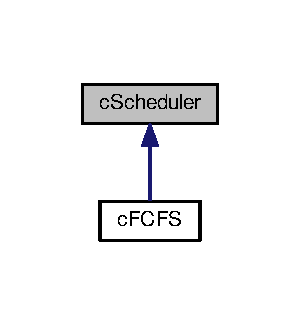
\includegraphics[width=350pt]{d8/dde/classcScheduler__inherit__graph}
\end{center}
\end{figure}
\subsection*{\-Public \-Member \-Functions}
\begin{DoxyCompactItemize}
\item 
virtual void \hyperlink{classcScheduler_a8782803287dce0352623142643eee01a}{init\-Proc\-Schedule\-Info} (\hyperlink{structProcessInfo}{\-Process\-Info} $\ast$)=0
\begin{DoxyCompactList}\small\item\em \-Initialize scheduler specific information within the \hyperlink{structProcessInfo}{\-Process\-Info} struct. \end{DoxyCompactList}\item 
virtual void \hyperlink{classcScheduler_aeae779c5c160a441e725dfc72656e6dc}{add\-Process} (\hyperlink{structProcessInfo}{\-Process\-Info} $\ast$)=0
\begin{DoxyCompactList}\small\item\em \-Transfer control of process state and scheduling. \end{DoxyCompactList}\item 
virtual void \hyperlink{classcScheduler_ae6119e940a3bf58a00e7dbcea04b5b6a}{set\-Blocked} (\hyperlink{structProcessInfo}{\-Process\-Info} $\ast$)=0
\begin{DoxyCompactList}\small\item\em \-Set a process into a \hyperlink{process_8h_a2c72cb00af5be695c1f898162350821fa035732e2026cb263f1bd9eee6ca6ae01}{blocked} state. \end{DoxyCompactList}\item 
virtual void \hyperlink{classcScheduler_a81fe2e5e5e2334e36db1cbf491e3fa57}{unblock\-Process} (\hyperlink{structProcessInfo}{\-Process\-Info} $\ast$)=0
\begin{DoxyCompactList}\small\item\em \-Unblock a process and make it ready. \end{DoxyCompactList}\item 
virtual void \hyperlink{classcScheduler_a5632ffa597e9567d475c808070c4e3bb}{remove\-Process} (\hyperlink{structProcessInfo}{\-Process\-Info} $\ast$)=0
\begin{DoxyCompactList}\small\item\em \-Remove a process from the control of the scheduler. \end{DoxyCompactList}\item 
virtual \hyperlink{structProcessInfo}{\-Process\-Info} $\ast$ \hyperlink{classcScheduler_a350ad7c55ddcdd17005778b0da241956}{get\-Next\-To\-Run} ()=0
\begin{DoxyCompactList}\small\item\em \-Query the scheduler for next process to run. \end{DoxyCompactList}\item 
virtual pid\-Type \hyperlink{classcScheduler_a025532a943093ae7e8d6dc0cdaf60f12}{num\-Processes} ()=0
\begin{DoxyCompactList}\small\item\em \-How many processes are in the scheduler. \end{DoxyCompactList}\item 
virtual void \hyperlink{classcScheduler_a7b29af7eab1a9cbe383d98a44693be69}{add\-Logger} (\-F\-I\-L\-E $\ast$)=0
\begin{DoxyCompactList}\small\item\em \-Add an instance of the trace logger to the scheduler. \end{DoxyCompactList}\item 
virtual void \hyperlink{classcScheduler_a3e7865112718057fcdc277db0a85c21c}{add\-Proc\-Logger} (\hyperlink{classcProcessLogger}{c\-Process\-Logger} $\ast$)=0
\begin{DoxyCompactList}\small\item\em \-Add instance of process logger to the scheduler. \end{DoxyCompactList}\item 
virtual void \hyperlink{classcScheduler_a27258d070a59a61a0b0ecbb35c514417}{print\-Unblocked} ()=0
\begin{DoxyCompactList}\small\item\em \-Prints at once all processes that may have become unblocked asynchronously. \end{DoxyCompactList}\end{DoxyCompactItemize}


\subsection{\-Member \-Function \-Documentation}
\hypertarget{classcScheduler_a7b29af7eab1a9cbe383d98a44693be69}{\index{c\-Scheduler@{c\-Scheduler}!add\-Logger@{add\-Logger}}
\index{add\-Logger@{add\-Logger}!cScheduler@{c\-Scheduler}}
\subsubsection[{add\-Logger}]{\setlength{\rightskip}{0pt plus 5cm}void {\bf c\-Scheduler\-::add\-Logger} (
\begin{DoxyParamCaption}
\item[{\-F\-I\-L\-E $\ast$}]{}
\end{DoxyParamCaption}
)\hspace{0.3cm}{\ttfamily  \mbox{[}pure virtual\mbox{]}}}}\label{d0/d21/classcScheduler_a7b29af7eab1a9cbe383d98a44693be69}
\-The kernel passes a file stream pointer for the scheduler to print trace info such as blocking/unblocking events.


\begin{DoxyParams}{\-Parameters}
{\em \-F\-I\-L\-E$\ast$} & \-File stream for trace log \\
\hline
\end{DoxyParams}
\begin{DoxySeeAlso}{\-See also}
\hyperlink{logger_8h_acf2f61176acdfe03ac9f73ec56fb3bd6}{init\-Log(const char$\ast$ filename)} 

\hyperlink{logger_8h_af756a6a1097f12014f446b298d8a266f}{get\-Stream()} 
\end{DoxySeeAlso}


\-Implemented in \hyperlink{classcMultiLevel_aa26aafd1e6a4582d16b47df72ca68601}{c\-Multi\-Level}, \hyperlink{classcRoundRobin_a6e0d0ec272a4f7ffe03166b1ff08276b}{c\-Round\-Robin}, \hyperlink{classcFCFS_accb887eae7016719ce770d7b0284adea}{c\-F\-C\-F\-S}, and \hyperlink{classcLottery_ad9b5803ea8dabd0df69d8063173b95a5}{c\-Lottery}.



\-Referenced by c\-Kernel\-::c\-Kernel().

\hypertarget{classcScheduler_aeae779c5c160a441e725dfc72656e6dc}{\index{c\-Scheduler@{c\-Scheduler}!add\-Process@{add\-Process}}
\index{add\-Process@{add\-Process}!cScheduler@{c\-Scheduler}}
\subsubsection[{add\-Process}]{\setlength{\rightskip}{0pt plus 5cm}void {\bf c\-Scheduler\-::add\-Process} (
\begin{DoxyParamCaption}
\item[{{\bf \-Process\-Info} $\ast$}]{}
\end{DoxyParamCaption}
)\hspace{0.3cm}{\ttfamily  \mbox{[}pure virtual\mbox{]}}}}\label{d0/d21/classcScheduler_aeae779c5c160a441e725dfc72656e6dc}
\-After this is called, the kernel core no longer keeps track of the given process. \-Once the process is created and deemed \hyperlink{process_8h_a2c72cb00af5be695c1f898162350821fa3d4001ca586c857718be397374082d76}{ready} by the kernel it is handed off here. \-The scheduler is then in charge of state transitions when the kernel gives it appropriate notifications.

\-Implementation \-Requirements\-: \begin{DoxyItemize}
\item \-Store the process in some location. \-It should be recognized as ready given its location but the datastructures and organization are implementation specific.\end{DoxyItemize}

\begin{DoxyParams}{\-Parameters}
{\em \-Process\-Info$\ast$} & \-Process to add under scheduler's control \\
\hline
\end{DoxyParams}


\-Implemented in \hyperlink{classcMultiLevel_af34029dd10cbd0b97d5c9f026e7c3838}{c\-Multi\-Level}, \hyperlink{classcRoundRobin_a3571d05a8daebccb758d63b8327f8a22}{c\-Round\-Robin}, \hyperlink{classcFCFS_a25d4bf440041f5294f3b9c5aff20b411}{c\-F\-C\-F\-S}, and \hyperlink{classcLottery_ae250b46d5d3032d40f49b8539cbd9faf}{c\-Lottery}.



\-Referenced by c\-Kernel\-::init\-Process().

\hypertarget{classcScheduler_a3e7865112718057fcdc277db0a85c21c}{\index{c\-Scheduler@{c\-Scheduler}!add\-Proc\-Logger@{add\-Proc\-Logger}}
\index{add\-Proc\-Logger@{add\-Proc\-Logger}!cScheduler@{c\-Scheduler}}
\subsubsection[{add\-Proc\-Logger}]{\setlength{\rightskip}{0pt plus 5cm}void {\bf c\-Scheduler\-::add\-Proc\-Logger} (
\begin{DoxyParamCaption}
\item[{{\bf c\-Process\-Logger} $\ast$}]{}
\end{DoxyParamCaption}
)\hspace{0.3cm}{\ttfamily  \mbox{[}pure virtual\mbox{]}}}}\label{d0/d21/classcScheduler_a3e7865112718057fcdc277db0a85c21c}
\-The kernel passes this pointer so the scheduler can update process info upon process addition, state change and termination. \-This updates the information presented to the top process.


\begin{DoxyParams}{\-Parameters}
{\em c\-Process\-Logger$\ast$} & \-Process logger class \\
\hline
\end{DoxyParams}
\begin{DoxySeeAlso}{\-See also}
\hyperlink{classcProcessLogger}{c\-Process\-Logger} 
\end{DoxySeeAlso}


\-Implemented in \hyperlink{classcMultiLevel_ad87a35e7828a916b4542c0fdd6301323}{c\-Multi\-Level}, \hyperlink{classcRoundRobin_a728fa415647d6c71b32ee8d4a04580e1}{c\-Round\-Robin}, \hyperlink{classcFCFS_a4da9f2fa83516ac5859772ae09169343}{c\-F\-C\-F\-S}, and \hyperlink{classcLottery_a3181bce7c9e3464215fdd9c328851787}{c\-Lottery}.



\-Referenced by c\-Kernel\-::c\-Kernel().

\hypertarget{classcScheduler_a350ad7c55ddcdd17005778b0da241956}{\index{c\-Scheduler@{c\-Scheduler}!get\-Next\-To\-Run@{get\-Next\-To\-Run}}
\index{get\-Next\-To\-Run@{get\-Next\-To\-Run}!cScheduler@{c\-Scheduler}}
\subsubsection[{get\-Next\-To\-Run}]{\setlength{\rightskip}{0pt plus 5cm}{\bf \-Process\-Info} $\ast$ {\bf c\-Scheduler\-::get\-Next\-To\-Run} (
\begin{DoxyParamCaption}
{}
\end{DoxyParamCaption}
)\hspace{0.3cm}{\ttfamily  \mbox{[}pure virtual\mbox{]}}}}\label{d0/d21/classcScheduler_a350ad7c55ddcdd17005778b0da241956}
\-After this function is called, it should be assumed by any scheduler implementation that the kernel will run the given process (unless otherwise notified). \-The currently running process should implicitly be considered for running next (again).

\-If there are processes left but all are blocked. \-This function should block until it receives a signal that a process is unblocked.

\-Implementation \-Requirements\-: \begin{DoxyItemize}
\item \-Call \hyperlink{classcScheduler_a27258d070a59a61a0b0ecbb35c514417}{print\-Unblocked()} to update the trace log after a clock step. \item \-Block if there are $>$ 0 processes but none can run. \item \-A process listed as \hyperlink{process_8h_a2c72cb00af5be695c1f898162350821faf9ccc71a0c4e71cc139d2c885154b243}{running} within the scheduler should be treated as ready when this method is called. \item \-A process returned as the 'next to run' should be marked as being in a \hyperlink{process_8h_a2c72cb00af5be695c1f898162350821faf9ccc71a0c4e71cc139d2c885154b243}{running} state before returning. \item \-If there are no more remaining processes this should return \-N\-U\-L\-L.\end{DoxyItemize}
\begin{DoxyReturn}{\-Returns}
\hyperlink{structProcessInfo}{\-Process\-Info}$\ast$ \-Ready process to run next. \-May be the same as the currenlty running one.
\end{DoxyReturn}
\begin{DoxyWarning}{\-Warning}
\-Must be thread safe with block and unblock methods. 
\end{DoxyWarning}


\-Implemented in \hyperlink{classcMultiLevel_af653d9a0d370d95c5d27914bae976628}{c\-Multi\-Level}, \hyperlink{classcRoundRobin_a1979ff71bb2320bdb00eae5feb2b2688}{c\-Round\-Robin}, \hyperlink{classcFCFS_aa2b92a8a992078e499aab455c9d78faf}{c\-F\-C\-F\-S}, and \hyperlink{classcLottery_a81195e7055070fa9743497621898c441}{c\-Lottery}.



\-Referenced by c\-Kernel\-::boot().

\hypertarget{classcScheduler_a8782803287dce0352623142643eee01a}{\index{c\-Scheduler@{c\-Scheduler}!init\-Proc\-Schedule\-Info@{init\-Proc\-Schedule\-Info}}
\index{init\-Proc\-Schedule\-Info@{init\-Proc\-Schedule\-Info}!cScheduler@{c\-Scheduler}}
\subsubsection[{init\-Proc\-Schedule\-Info}]{\setlength{\rightskip}{0pt plus 5cm}void {\bf c\-Scheduler\-::init\-Proc\-Schedule\-Info} (
\begin{DoxyParamCaption}
\item[{{\bf \-Process\-Info} $\ast$}]{}
\end{DoxyParamCaption}
)\hspace{0.3cm}{\ttfamily  \mbox{[}pure virtual\mbox{]}}}}\label{d0/d21/classcScheduler_a8782803287dce0352623142643eee01a}
\-This method is called after the kernel has initialized all process data but before it is marked \hyperlink{process_8h_a2c72cb00af5be695c1f898162350821fa3d4001ca586c857718be397374082d76}{ready}. \-This gives the scheduler an oportunity to initialize any scheduler specific data and assign it to the \hyperlink{structProcessInfo_aea1c50ae92f6421ae5c94ac674c1877a}{\-Process\-Info\-::schedule\-Data} member.

\-Implementation \-Requirements\-: \begin{DoxyItemize}
\item \-No required actions. \end{DoxyItemize}


\-Implemented in \hyperlink{classcMultiLevel_ad403c4589bcd66289aa0c9f6a78a7a1b}{c\-Multi\-Level}, \hyperlink{classcRoundRobin_aadb221df9b12f61c3151996ea5c09741}{c\-Round\-Robin}, \hyperlink{classcFCFS_aff34f18c6f4c3f38029d904cd2ec55de}{c\-F\-C\-F\-S}, and \hyperlink{classcLottery_a04e2ae003310bf45f0db0d3017e308e2}{c\-Lottery}.



\-Referenced by c\-Kernel\-::init\-Process().

\hypertarget{classcScheduler_a025532a943093ae7e8d6dc0cdaf60f12}{\index{c\-Scheduler@{c\-Scheduler}!num\-Processes@{num\-Processes}}
\index{num\-Processes@{num\-Processes}!cScheduler@{c\-Scheduler}}
\subsubsection[{num\-Processes}]{\setlength{\rightskip}{0pt plus 5cm}pid\-Type {\bf c\-Scheduler\-::num\-Processes} (
\begin{DoxyParamCaption}
{}
\end{DoxyParamCaption}
)\hspace{0.3cm}{\ttfamily  \mbox{[}pure virtual\mbox{]}}}}\label{d0/d21/classcScheduler_a025532a943093ae7e8d6dc0cdaf60f12}
\-This returns how many processes, both running and blocked, are being handled by the scheduler.

\-Implementation \-Requirements\-: \begin{DoxyItemize}
\item \-Return how many processes, running and blocked, are in the scheduler.\end{DoxyItemize}
\begin{DoxyReturn}{\-Returns}
pid\-Type 
\end{DoxyReturn}


\-Implemented in \hyperlink{classcMultiLevel_ab36db79f48f6dd388eb8504af261d3e4}{c\-Multi\-Level}, \hyperlink{classcRoundRobin_afa0cdfcfc0b8222d39ad5e9c23db1f25}{c\-Round\-Robin}, \hyperlink{classcFCFS_a0a72de791436a84120a534dd2fa0485d}{c\-F\-C\-F\-S}, and \hyperlink{classcLottery_a4f77d186c1f4cbb82d3fff077bba7736}{c\-Lottery}.



\-Referenced by c\-Kernel\-::boot(), and c\-Kernel\-::c\-Kernel().

\hypertarget{classcScheduler_a27258d070a59a61a0b0ecbb35c514417}{\index{c\-Scheduler@{c\-Scheduler}!print\-Unblocked@{print\-Unblocked}}
\index{print\-Unblocked@{print\-Unblocked}!cScheduler@{c\-Scheduler}}
\subsubsection[{print\-Unblocked}]{\setlength{\rightskip}{0pt plus 5cm}void {\bf c\-Scheduler\-::print\-Unblocked} (
\begin{DoxyParamCaption}
{}
\end{DoxyParamCaption}
)\hspace{0.3cm}{\ttfamily  \mbox{[}pure virtual\mbox{]}}}}\label{d0/d21/classcScheduler_a27258d070a59a61a0b0ecbb35c514417}
\-This method is needed to avoid mixed output in the trace logger. 

\-Implemented in \hyperlink{classcMultiLevel_a3e20033afe7915530ad5fc4c9baf0a70}{c\-Multi\-Level}, \hyperlink{classcRoundRobin_a3df89085fb98c328b7db6bfc0ee9f9f9}{c\-Round\-Robin}, \hyperlink{classcFCFS_a37af1bbb7393f800a24ff22ee443f876}{c\-F\-C\-F\-S}, and \hyperlink{classcLottery_ab878165e4106b7e09cfa1fbc87d33d1b}{c\-Lottery}.

\hypertarget{classcScheduler_a5632ffa597e9567d475c808070c4e3bb}{\index{c\-Scheduler@{c\-Scheduler}!remove\-Process@{remove\-Process}}
\index{remove\-Process@{remove\-Process}!cScheduler@{c\-Scheduler}}
\subsubsection[{remove\-Process}]{\setlength{\rightskip}{0pt plus 5cm}void {\bf c\-Scheduler\-::remove\-Process} (
\begin{DoxyParamCaption}
\item[{{\bf \-Process\-Info} $\ast$}]{}
\end{DoxyParamCaption}
)\hspace{0.3cm}{\ttfamily  \mbox{[}pure virtual\mbox{]}}}}\label{d0/d21/classcScheduler_a5632ffa597e9567d475c808070c4e3bb}
\-When a process terminates, either through normal means or an exception, the kernel will call this function to release a process from the scheduler's control. \-The scheduler should clean up any internal state for the process. \-Deallocation of process resources is left to the kernel.

\-Implementation \-Requirements\-: \begin{DoxyItemize}
\item \-Scheduler should deallocate any resources it assigned to the process within the \hyperlink{structProcessInfo_aea1c50ae92f6421ae5c94ac674c1877a}{\-Process\-Info\-::schedule\-Data} member. \item \-The \-Scheduler should remove any pointers to the give process to avoid dereferncing a dead pointer. \item \-Implementations must not deallocate any memory except that mentioned above. \-This is handled by the kernel. \item \-Implementations should mark the process as \hyperlink{process_8h_a2c72cb00af5be695c1f898162350821fa21b6f86c6d8b11d4a9c163130f55c5dd}{terminated}.\end{DoxyItemize}

\begin{DoxyParams}{\-Parameters}
{\em \-Process\-Info$\ast$} & \-Process to remove from scheduler \\
\hline
\end{DoxyParams}


\-Implemented in \hyperlink{classcMultiLevel_a862a0b03ba06e25021486aa396446895}{c\-Multi\-Level}, \hyperlink{classcRoundRobin_a1bc7bfc4c36bdbe3f3938810817d885e}{c\-Round\-Robin}, \hyperlink{classcFCFS_aeeac757885108ae510b728600ebba248}{c\-F\-C\-F\-S}, and \hyperlink{classcLottery_aa995fc5a68b398aa526e504fed2f7a59}{c\-Lottery}.



\-Referenced by c\-Kernel\-::cleanup\-Process().

\hypertarget{classcScheduler_ae6119e940a3bf58a00e7dbcea04b5b6a}{\index{c\-Scheduler@{c\-Scheduler}!set\-Blocked@{set\-Blocked}}
\index{set\-Blocked@{set\-Blocked}!cScheduler@{c\-Scheduler}}
\subsubsection[{set\-Blocked}]{\setlength{\rightskip}{0pt plus 5cm}void {\bf c\-Scheduler\-::set\-Blocked} (
\begin{DoxyParamCaption}
\item[{{\bf \-Process\-Info} $\ast$}]{}
\end{DoxyParamCaption}
)\hspace{0.3cm}{\ttfamily  \mbox{[}pure virtual\mbox{]}}}}\label{d0/d21/classcScheduler_ae6119e940a3bf58a00e7dbcea04b5b6a}
\-The kernel will call the scheduler with this function when the process has done an operation which causes it to block (\-I).

\-Implementation \-Requirements\-: \begin{DoxyItemize}
\item \-Process must be marked \hyperlink{process_8h_a2c72cb00af5be695c1f898162350821fa035732e2026cb263f1bd9eee6ca6ae01}{blocked} and scheduler state should be changed accordingly. \item \-After this call a process should not be considered for a scheduling decision\end{DoxyItemize}
\begin{DoxyWarning}{\-Warning}
\-Must be thread safe. \-Signal handler/s may block during schedule decision. 
\end{DoxyWarning}


\-Implemented in \hyperlink{classcMultiLevel_a2d3f9e5013d5ef2777c64aa662f98fbd}{c\-Multi\-Level}, \hyperlink{classcRoundRobin_a13609de0f36c81a780072f9c0730f963}{c\-Round\-Robin}, \hyperlink{classcFCFS_a1b8ee3a759a31032ec7c1cd7b15ed5df}{c\-F\-C\-F\-S}, and \hyperlink{classcLottery_afa726859adb7b98f1ad80a41c196e488}{c\-Lottery}.



\-Referenced by c\-Kernel\-::boot().

\hypertarget{classcScheduler_a81fe2e5e5e2334e36db1cbf491e3fa57}{\index{c\-Scheduler@{c\-Scheduler}!unblock\-Process@{unblock\-Process}}
\index{unblock\-Process@{unblock\-Process}!cScheduler@{c\-Scheduler}}
\subsubsection[{unblock\-Process}]{\setlength{\rightskip}{0pt plus 5cm}void {\bf c\-Scheduler\-::unblock\-Process} (
\begin{DoxyParamCaption}
\item[{{\bf \-Process\-Info} $\ast$}]{}
\end{DoxyParamCaption}
)\hspace{0.3cm}{\ttfamily  \mbox{[}pure virtual\mbox{]}}}}\label{d0/d21/classcScheduler_a81fe2e5e5e2334e36db1cbf491e3fa57}
\-When a process has completed a blocking call the kernel will notify the scheduler that it should be unblocked. \-This operation should be very fast since it will likely be called from a signal handler.

\-Implementation \-Requirements\-: \begin{DoxyItemize}
\item \-The process must be unblocked and marked \hyperlink{process_8h_a2c72cb00af5be695c1f898162350821fa3d4001ca586c857718be397374082d76}{ready}. \-It must be available for scheduling with the next call to \-::get\-Next\-To\-Run\end{DoxyItemize}

\begin{DoxyParams}{\-Parameters}
{\em \-Process\-Info$\ast$} & \-Process to unblock\\
\hline
\end{DoxyParams}
\begin{DoxyWarning}{\-Warning}
\-Must be thread safe. \-Signal handler/s may unblock during schedule decision. 
\end{DoxyWarning}


\-Implemented in \hyperlink{classcMultiLevel_abe3cfe3c2a5828505ea5c52fb12f7d09}{c\-Multi\-Level}, \hyperlink{classcRoundRobin_a278d541c78f034020f6921b22a7d37af}{c\-Round\-Robin}, \hyperlink{classcFCFS_a793da0298f9b36ab8505a0e3daaf41ec}{c\-F\-C\-F\-S}, and \hyperlink{classcLottery_a86bf3ddc6da1a45ffb073a843d744c60}{c\-Lottery}.



\-The documentation for this class was generated from the following file\-:\begin{DoxyCompactItemize}
\item 
include/scheduler/scheduler.\-h\end{DoxyCompactItemize}

\hypertarget{structfcfsInfo}{\section{fcfs\-Info \-Struct \-Reference}
\label{d5/d4c/structfcfsInfo}\index{fcfs\-Info@{fcfs\-Info}}
}


\-Struct containing process info specific for \-F\-C\-F\-S scheduling.  




{\ttfamily \#include $<$fcfs.\-h$>$}

\subsection*{\-Public \-Attributes}
\begin{DoxyCompactItemize}
\item 
\hypertarget{structfcfsInfo_a994331c8dd9b432273d61e44e17807fd}{unsigned int {\bfseries blocked\-Index}}\label{d5/d4c/structfcfsInfo_a994331c8dd9b432273d61e44e17807fd}

\end{DoxyCompactItemize}


\-The documentation for this struct was generated from the following file\-:\begin{DoxyCompactItemize}
\item 
include/scheduler/\hyperlink{fcfs_8h}{fcfs.\-h}\end{DoxyCompactItemize}

\hypertarget{structkernelError}{\section{kernel\-Error \-Struct \-Reference}
\label{dc/d4b/structkernelError}\index{kernel\-Error@{kernel\-Error}}
}


\-Struct containing kernel crash information.  




{\ttfamily \#include $<$kernel.\-h$>$}



\-Collaboration diagram for kernel\-Error\-:\nopagebreak
\begin{figure}[H]
\begin{center}
\leavevmode
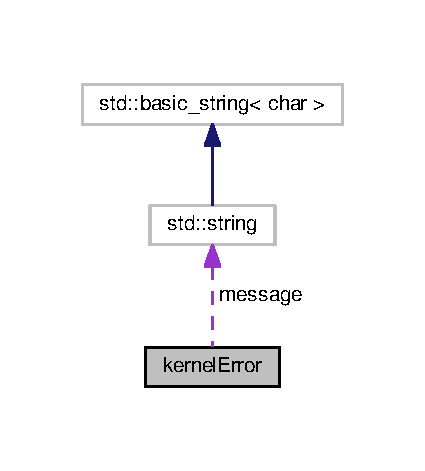
\includegraphics[width=204pt]{dc/df6/structkernelError__coll__graph}
\end{center}
\end{figure}
\subsection*{\-Public \-Attributes}
\begin{DoxyCompactItemize}
\item 
\hypertarget{structkernelError_a047e3e93719a3267825e891fe9285981}{string {\bfseries message}}\label{dc/d4b/structkernelError_a047e3e93719a3267825e891fe9285981}

\end{DoxyCompactItemize}


\subsection{\-Detailed \-Description}
\-When the kernel crashes, important information is placed in here and then handled by the main function in init.\-cpp. 

\-The documentation for this struct was generated from the following file\-:\begin{DoxyCompactItemize}
\item 
include/\hyperlink{kernel_8h}{kernel.\-h}\end{DoxyCompactItemize}

\hypertarget{structProcessInfo}{\section{\-Process\-Info \-Struct \-Reference}
\label{dd/dc8/structProcessInfo}\index{\-Process\-Info@{\-Process\-Info}}
}


\-Structure for containing process state and data.  




{\ttfamily \#include $<$process.\-h$>$}

\subsection*{\-Public \-Attributes}
\begin{DoxyCompactItemize}
\item 
\hypertarget{structProcessInfo_a102b9e7e7d958b508cec182bbcaf7d85}{unsigned int {\bfseries parent}}\label{dd/dc8/structProcessInfo_a102b9e7e7d958b508cec182bbcaf7d85}

\item 
\hypertarget{structProcessInfo_ab522cec1e6f7f3b6a7780e6b4611c1f4}{unsigned int {\bfseries pid}}\label{dd/dc8/structProcessInfo_ab522cec1e6f7f3b6a7780e6b4611c1f4}

\item 
\hypertarget{structProcessInfo_ac1e6244dd31274040bdf7ad7ee40db4a}{unsigned int {\bfseries start\-C\-P\-U}}\label{dd/dc8/structProcessInfo_ac1e6244dd31274040bdf7ad7ee40db4a}

\item 
\hypertarget{structProcessInfo_a8a6eda10132e07b1596c09822724b0c7}{unsigned int {\bfseries total\-C\-P\-U}}\label{dd/dc8/structProcessInfo_a8a6eda10132e07b1596c09822724b0c7}

\item 
\hypertarget{structProcessInfo_a748790bb8c3ef5d2dff552f35b81298e}{\hyperlink{process_8h_a2c72cb00af5be695c1f898162350821f}{e\-Proc\-State} \hyperlink{structProcessInfo_a748790bb8c3ef5d2dff552f35b81298e}{state}}\label{dd/dc8/structProcessInfo_a748790bb8c3ef5d2dff552f35b81298e}

\begin{DoxyCompactList}\small\item\em \hyperlink{process_8h_a2c72cb00af5be695c1f898162350821f}{e\-Proc\-State} \end{DoxyCompactList}\item 
\hypertarget{structProcessInfo_af818acf9075de7c0100858908bcc2867}{uint16\-\_\-t {\bfseries \-P\-S\-W}}\label{dd/dc8/structProcessInfo_af818acf9075de7c0100858908bcc2867}

\item 
\hypertarget{structProcessInfo_a2f9f55dc3548d0bed66e06db8f47d958}{int {\bfseries priority}}\label{dd/dc8/structProcessInfo_a2f9f55dc3548d0bed66e06db8f47d958}

\item 
\hypertarget{structProcessInfo_a9b2d3f321f21ec1ee97c8dd5e63ac6c8}{unsigned int {\bfseries \-P\-C}}\label{dd/dc8/structProcessInfo_a9b2d3f321f21ec1ee97c8dd5e63ac6c8}

\item 
\hypertarget{structProcessInfo_ab288b59e794cb506663e22c680e05c2d}{int {\bfseries \-V\-C}}\label{dd/dc8/structProcessInfo_ab288b59e794cb506663e22c680e05c2d}

\item 
\hypertarget{structProcessInfo_ae99b529cb79a446c0ff0d1a851b67fc5}{char $\ast$ {\bfseries process\-Text}}\label{dd/dc8/structProcessInfo_ae99b529cb79a446c0ff0d1a851b67fc5}

\item 
\hypertarget{structProcessInfo_aea1c50ae92f6421ae5c94ac674c1877a}{void $\ast$ {\bfseries schedule\-Data}}\label{dd/dc8/structProcessInfo_aea1c50ae92f6421ae5c94ac674c1877a}

\item 
\hypertarget{structProcessInfo_aa65ed051998c0493b68feeea5ae4955f}{unsigned long {\bfseries memory}}\label{dd/dc8/structProcessInfo_aa65ed051998c0493b68feeea5ae4955f}

\end{DoxyCompactItemize}


\subsection{\-Detailed \-Description}
\-This struture is created in the kernel when a process is initialized. \-It contains all process data needed for execution and for the kernel/scheduler to make desciions on it. 

\-The documentation for this struct was generated from the following file\-:\begin{DoxyCompactItemize}
\item 
include/\hyperlink{process_8h}{process.\-h}\end{DoxyCompactItemize}

\chapter{\-File \-Documentation}
\hypertarget{cpu_8h}{\section{include/cpu.h \-File \-Reference}
\label{dc/da7/cpu_8h}\index{include/cpu.\-h@{include/cpu.\-h}}
}
{\ttfamily \#include $<$cstdio$>$}\*
{\ttfamily \#include $<$cstdlib$>$}\*
{\ttfamily \#include $<$assert.\-h$>$}\*
{\ttfamily \#include $<$inttypes.\-h$>$}\*
\-Include dependency graph for cpu.\-h\-:\nopagebreak
\begin{figure}[H]
\begin{center}
\leavevmode
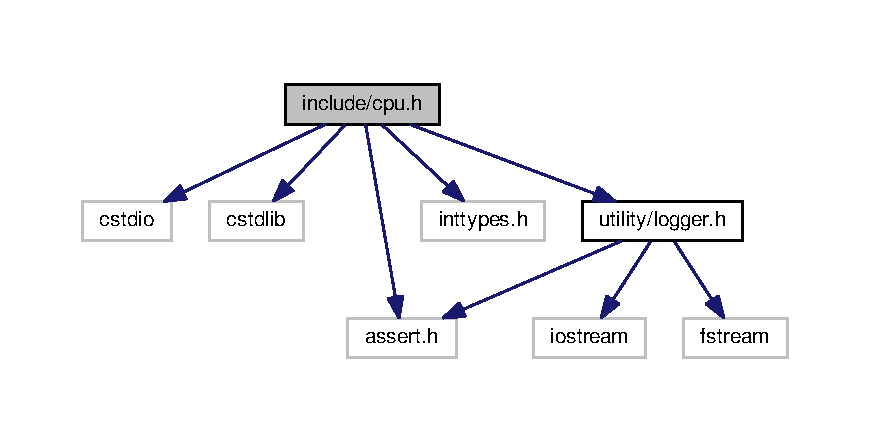
\includegraphics[width=333pt]{d4/d37/cpu_8h__incl}
\end{center}
\end{figure}
\-This graph shows which files directly or indirectly include this file\-:\nopagebreak
\begin{figure}[H]
\begin{center}
\leavevmode
\includegraphics[width=164pt]{d8/de6/cpu_8h__dep__incl}
\end{center}
\end{figure}
\subsection*{\-Classes}
\begin{DoxyCompactItemize}
\item 
class \hyperlink{classcCPU}{c\-C\-P\-U}
\begin{DoxyCompactList}\small\item\em \-A class for emulating a simple cpu. \end{DoxyCompactList}\end{DoxyCompactItemize}
\subsection*{\-Defines}
\begin{DoxyCompactItemize}
\item 
\hypertarget{cpu_8h_a885a6481fc6d474d0be18bc0facf648d}{\#define \hyperlink{cpu_8h_a885a6481fc6d474d0be18bc0facf648d}{\-M\-A\-X\-\_\-\-P\-A\-R\-A\-M\-S}~2}\label{dc/da7/cpu_8h_a885a6481fc6d474d0be18bc0facf648d}

\begin{DoxyCompactList}\small\item\em \-Max number of execution parameters for any \-Opcode. \end{DoxyCompactList}\item 
\#define \hyperlink{cpu_8h_a9e34e5196b1f8e4c96f229d062c73fe0}{\-M\-A\-X\-\_\-\-P\-A\-R\-A\-M\-\_\-\-S\-I\-Z\-E}~256
\begin{DoxyCompactList}\small\item\em \-Maximum size in bytes for an execution parameter. \end{DoxyCompactList}\end{DoxyCompactItemize}
\subsection*{\-Enumerations}
\begin{DoxyCompactItemize}
\item 
enum \hyperlink{cpu_8h_ade10811b11f1c647313bf0a60797a9f9}{e\-P\-S\-W} \{ \hyperlink{cpu_8h_ade10811b11f1c647313bf0a60797a9f9a5f0829985f41a81da1a46db3501075f1}{\-P\-S\-\_\-\-E\-X\-C\-E\-P\-T\-I\-O\-N} =  0x1, 
\hyperlink{cpu_8h_ade10811b11f1c647313bf0a60797a9f9a45657e0129f354aef59ae454ef5443fd}{\-P\-S\-\_\-\-T\-E\-R\-M\-I\-N\-A\-T\-E} =  \-P\-S\-\_\-\-E\-X\-C\-E\-P\-T\-I\-O\-N $<$$<$ 1, 
\hyperlink{cpu_8h_ade10811b11f1c647313bf0a60797a9f9aa95675f79e2e3167dc1622eaf4733cee}{\-P\-S\-\_\-\-S\-Y\-S\-C\-A\-L\-L} =  \-P\-S\-\_\-\-T\-E\-R\-M\-I\-N\-A\-T\-E $<$$<$ 1
 \}
\begin{DoxyCompactList}\small\item\em \-Enumeration of \-Program \-Status \-Word \-Flags. \end{DoxyCompactList}\end{DoxyCompactItemize}


\subsection{\-Detailed \-Description}


\subsection{\-Define \-Documentation}
\hypertarget{cpu_8h_a9e34e5196b1f8e4c96f229d062c73fe0}{\index{cpu.\-h@{cpu.\-h}!\-M\-A\-X\-\_\-\-P\-A\-R\-A\-M\-\_\-\-S\-I\-Z\-E@{\-M\-A\-X\-\_\-\-P\-A\-R\-A\-M\-\_\-\-S\-I\-Z\-E}}
\index{\-M\-A\-X\-\_\-\-P\-A\-R\-A\-M\-\_\-\-S\-I\-Z\-E@{\-M\-A\-X\-\_\-\-P\-A\-R\-A\-M\-\_\-\-S\-I\-Z\-E}!cpu.h@{cpu.\-h}}
\subsubsection[{\-M\-A\-X\-\_\-\-P\-A\-R\-A\-M\-\_\-\-S\-I\-Z\-E}]{\setlength{\rightskip}{0pt plus 5cm}\#define {\bf \-M\-A\-X\-\_\-\-P\-A\-R\-A\-M\-\_\-\-S\-I\-Z\-E}~256}}\label{dc/da7/cpu_8h_a9e34e5196b1f8e4c96f229d062c73fe0}
\-Creates exception if exceeded. 

\subsection{\-Enumeration \-Type \-Documentation}
\hypertarget{cpu_8h_ade10811b11f1c647313bf0a60797a9f9}{\index{cpu.\-h@{cpu.\-h}!e\-P\-S\-W@{e\-P\-S\-W}}
\index{e\-P\-S\-W@{e\-P\-S\-W}!cpu.h@{cpu.\-h}}
\subsubsection[{e\-P\-S\-W}]{\setlength{\rightskip}{0pt plus 5cm}enum {\bf e\-P\-S\-W}}}\label{dc/da7/cpu_8h_ade10811b11f1c647313bf0a60797a9f9}
\-The program status word is a bit vector and this enumeration defines the meaning of particular bits. \-This is used in the interpretation of execution status. \begin{Desc}
\item[\-Enumerator\-: ]\par
\begin{description}
\index{\-P\-S\-\_\-\-E\-X\-C\-E\-P\-T\-I\-O\-N@{\-P\-S\-\_\-\-E\-X\-C\-E\-P\-T\-I\-O\-N}!cpu.\-h@{cpu.\-h}}\index{cpu.\-h@{cpu.\-h}!\-P\-S\-\_\-\-E\-X\-C\-E\-P\-T\-I\-O\-N@{\-P\-S\-\_\-\-E\-X\-C\-E\-P\-T\-I\-O\-N}}\item[{\em 
\hypertarget{cpu_8h_ade10811b11f1c647313bf0a60797a9f9a5f0829985f41a81da1a46db3501075f1}{\-P\-S\-\_\-\-E\-X\-C\-E\-P\-T\-I\-O\-N}\label{dc/da7/cpu_8h_ade10811b11f1c647313bf0a60797a9f9a5f0829985f41a81da1a46db3501075f1}
}]\-Executing process has created an exception. \index{\-P\-S\-\_\-\-T\-E\-R\-M\-I\-N\-A\-T\-E@{\-P\-S\-\_\-\-T\-E\-R\-M\-I\-N\-A\-T\-E}!cpu.\-h@{cpu.\-h}}\index{cpu.\-h@{cpu.\-h}!\-P\-S\-\_\-\-T\-E\-R\-M\-I\-N\-A\-T\-E@{\-P\-S\-\_\-\-T\-E\-R\-M\-I\-N\-A\-T\-E}}\item[{\em 
\hypertarget{cpu_8h_ade10811b11f1c647313bf0a60797a9f9a45657e0129f354aef59ae454ef5443fd}{\-P\-S\-\_\-\-T\-E\-R\-M\-I\-N\-A\-T\-E}\label{dc/da7/cpu_8h_ade10811b11f1c647313bf0a60797a9f9a45657e0129f354aef59ae454ef5443fd}
}]\-Executing process has finished. \index{\-P\-S\-\_\-\-S\-Y\-S\-C\-A\-L\-L@{\-P\-S\-\_\-\-S\-Y\-S\-C\-A\-L\-L}!cpu.\-h@{cpu.\-h}}\index{cpu.\-h@{cpu.\-h}!\-P\-S\-\_\-\-S\-Y\-S\-C\-A\-L\-L@{\-P\-S\-\_\-\-S\-Y\-S\-C\-A\-L\-L}}\item[{\em 
\hypertarget{cpu_8h_ade10811b11f1c647313bf0a60797a9f9aa95675f79e2e3167dc1622eaf4733cee}{\-P\-S\-\_\-\-S\-Y\-S\-C\-A\-L\-L}\label{dc/da7/cpu_8h_ade10811b11f1c647313bf0a60797a9f9aa95675f79e2e3167dc1622eaf4733cee}
}]\-Executing process has made a system call. \end{description}
\end{Desc}


\hypertarget{block__device_8h}{\section{include/devices/block\-\_\-device.h \-File \-Reference}
\label{db/d9a/block__device_8h}\index{include/devices/block\-\_\-device.\-h@{include/devices/block\-\_\-device.\-h}}
}
{\ttfamily \#include $<$cstdio$>$}\*
{\ttfamily \#include \char`\"{}devices/queued\-\_\-device.\-h\char`\"{}}\*
\-Include dependency graph for block\-\_\-device.\-h\-:\nopagebreak
\begin{figure}[H]
\begin{center}
\leavevmode
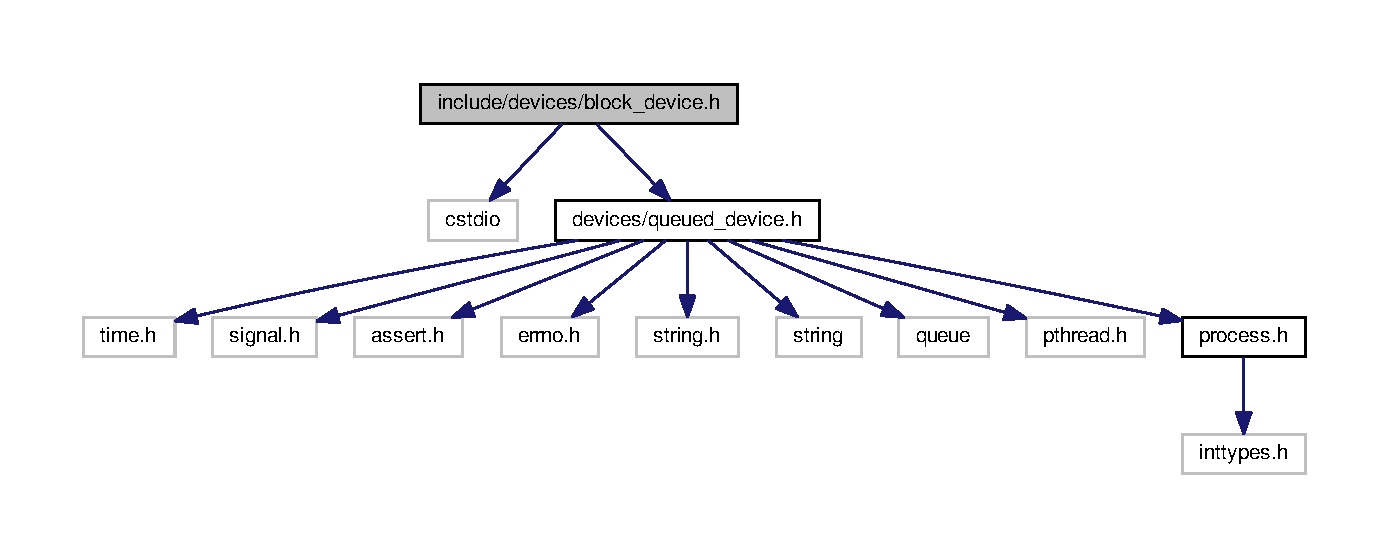
\includegraphics[width=350pt]{d7/d64/block__device_8h__incl}
\end{center}
\end{figure}
\-This graph shows which files directly or indirectly include this file\-:\nopagebreak
\begin{figure}[H]
\begin{center}
\leavevmode
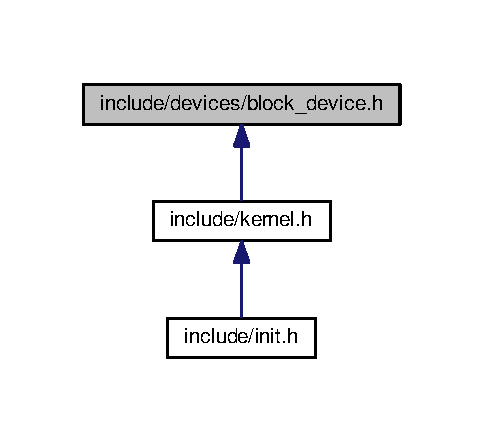
\includegraphics[width=232pt]{df/dd1/block__device_8h__dep__incl}
\end{center}
\end{figure}
\subsection*{\-Classes}
\begin{DoxyCompactItemize}
\item 
class \hyperlink{classcBlockDevice}{c\-Block\-Device}
\begin{DoxyCompactList}\small\item\em \-Queued block device. \end{DoxyCompactList}\end{DoxyCompactItemize}
\subsection*{\-Defines}
\begin{DoxyCompactItemize}
\item 
\hypertarget{block__device_8h_a40b115b8cd111feee88bd339876e7941}{\#define \hyperlink{block__device_8h_a40b115b8cd111feee88bd339876e7941}{\-B\-L\-O\-C\-K\-S\-I\-G}~\-S\-I\-G\-R\-T\-M\-I\-N + 1}\label{db/d9a/block__device_8h_a40b115b8cd111feee88bd339876e7941}

\begin{DoxyCompactList}\small\item\em \-Signal generated by \-Block\-Device. \end{DoxyCompactList}\end{DoxyCompactItemize}


\subsection{\-Detailed \-Description}

\hypertarget{char__device_8h}{\section{include/devices/char\-\_\-device.h \-File \-Reference}
\label{d7/d59/char__device_8h}\index{include/devices/char\-\_\-device.\-h@{include/devices/char\-\_\-device.\-h}}
}
{\ttfamily \#include \char`\"{}devices/queued\-\_\-device.\-h\char`\"{}}\*
\-Include dependency graph for char\-\_\-device.\-h\-:\nopagebreak
\begin{figure}[H]
\begin{center}
\leavevmode
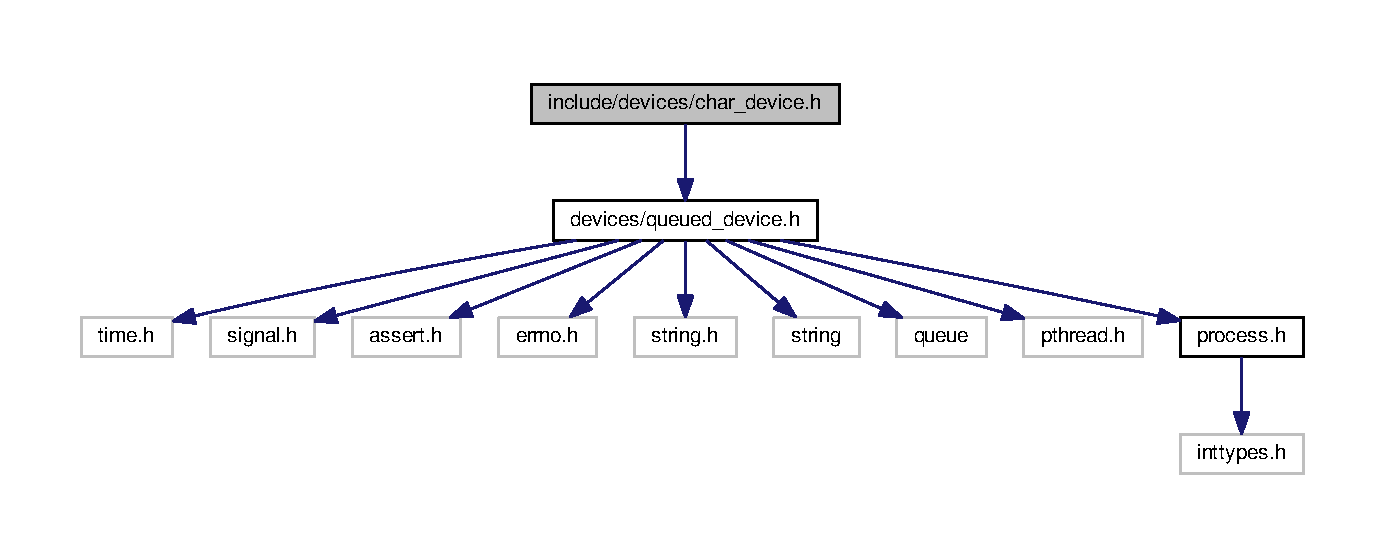
\includegraphics[width=350pt]{da/d18/char__device_8h__incl}
\end{center}
\end{figure}
\-This graph shows which files directly or indirectly include this file\-:\nopagebreak
\begin{figure}[H]
\begin{center}
\leavevmode
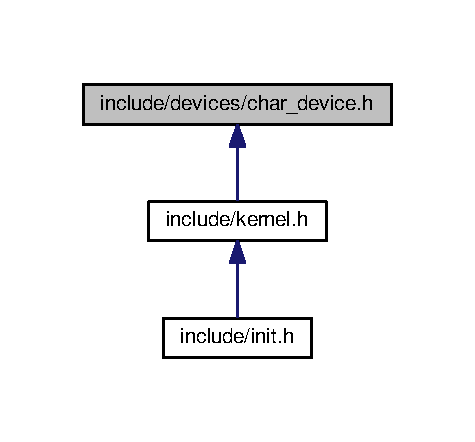
\includegraphics[width=228pt]{db/ded/char__device_8h__dep__incl}
\end{center}
\end{figure}
\subsection*{\-Classes}
\begin{DoxyCompactItemize}
\item 
class \hyperlink{classcCharDevice}{c\-Char\-Device}
\begin{DoxyCompactList}\small\item\em \-Queued char device. \end{DoxyCompactList}\end{DoxyCompactItemize}
\subsection*{\-Defines}
\begin{DoxyCompactItemize}
\item 
\hypertarget{char__device_8h_a2e6614e57b804a24ff80f29b9e840788}{\#define \hyperlink{char__device_8h_a2e6614e57b804a24ff80f29b9e840788}{\-C\-H\-A\-R\-S\-I\-G}~\-S\-I\-G\-R\-T\-M\-I\-N + 2}\label{d7/d59/char__device_8h_a2e6614e57b804a24ff80f29b9e840788}

\begin{DoxyCompactList}\small\item\em \-Signal generated by \-Char\-Device. \end{DoxyCompactList}\end{DoxyCompactItemize}


\subsection{\-Detailed \-Description}

\hypertarget{clock__device_8h}{\section{include/devices/clock\-\_\-device.h \-File \-Reference}
\label{df/d8f/clock__device_8h}\index{include/devices/clock\-\_\-device.\-h@{include/devices/clock\-\_\-device.\-h}}
}
{\ttfamily \#include $<$errno.\-h$>$}\*
{\ttfamily \#include $<$cstring$>$}\*
{\ttfamily \#include $<$string$>$}\*
{\ttfamily \#include \char`\"{}devices/abstract\-\_\-device.\-h\char`\"{}}\*
\-Include dependency graph for clock\-\_\-device.\-h\-:\nopagebreak
\begin{figure}[H]
\begin{center}
\leavevmode
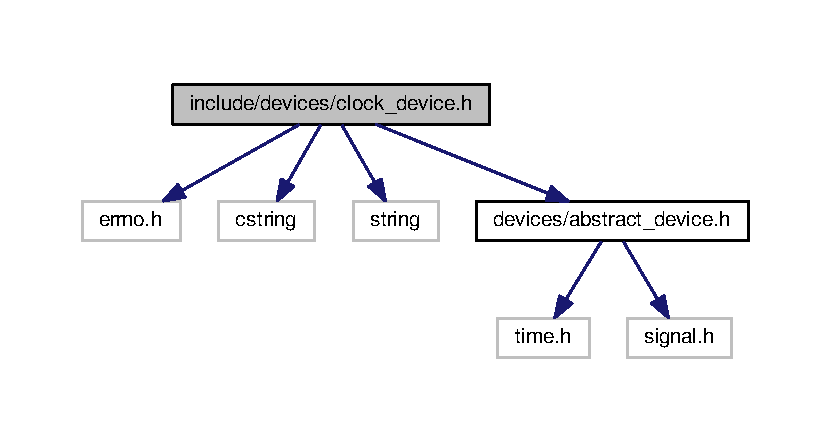
\includegraphics[width=350pt]{db/d16/clock__device_8h__incl}
\end{center}
\end{figure}
\-This graph shows which files directly or indirectly include this file\-:\nopagebreak
\begin{figure}[H]
\begin{center}
\leavevmode
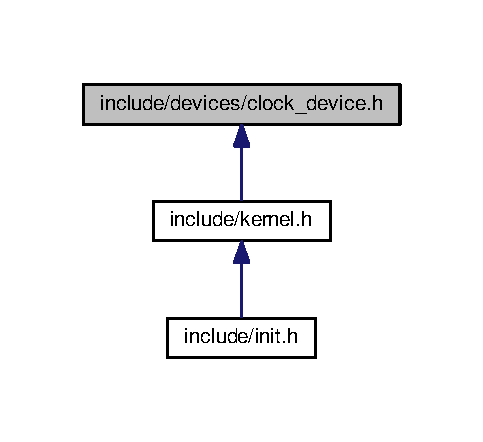
\includegraphics[width=232pt]{d8/d7f/clock__device_8h__dep__incl}
\end{center}
\end{figure}
\subsection*{\-Classes}
\begin{DoxyCompactItemize}
\item 
class \hyperlink{classClockDevice}{\-Clock\-Device}
\end{DoxyCompactItemize}
\subsection*{\-Defines}
\begin{DoxyCompactItemize}
\item 
\hypertarget{clock__device_8h_a2694a39dfd1fa087ca6f9f391c91dae7}{\#define {\bfseries \-C\-L\-O\-C\-K\-I\-D}~\-C\-L\-O\-C\-K\-\_\-\-R\-E\-A\-L\-T\-I\-M\-E}\label{df/d8f/clock__device_8h_a2694a39dfd1fa087ca6f9f391c91dae7}

\item 
\hypertarget{clock__device_8h_af6318deadd0687fb8ffb5437eaa1870d}{\#define \hyperlink{clock__device_8h_af6318deadd0687fb8ffb5437eaa1870d}{\-C\-L\-O\-C\-K\-S\-I\-G}~\-S\-I\-G\-R\-T\-M\-I\-N}\label{df/d8f/clock__device_8h_af6318deadd0687fb8ffb5437eaa1870d}

\begin{DoxyCompactList}\small\item\em \-Signal generated by \hyperlink{classClockDevice}{\-Clock\-Device}. \end{DoxyCompactList}\end{DoxyCompactItemize}


\subsection{\-Detailed \-Description}

\hypertarget{kernel_8h}{\section{include/kernel.h \-File \-Reference}
\label{d0/daa/kernel_8h}\index{include/kernel.\-h@{include/kernel.\-h}}
}
{\ttfamily \#include $<$vector$>$}\*
{\ttfamily \#include $<$fcntl.\-h$>$}\*
{\ttfamily \#include $<$sys/types.\-h$>$}\*
{\ttfamily \#include $<$sys/stat.\-h$>$}\*
{\ttfamily \#include \char`\"{}cpu.\-h\char`\"{}}\*
{\ttfamily \#include \char`\"{}devices/char\-\_\-device.\-h\char`\"{}}\*
{\ttfamily \#include \char`\"{}devices/block\-\_\-device.\-h\char`\"{}}\*
{\ttfamily \#include \char`\"{}devices/clock\-\_\-device.\-h\char`\"{}}\*
{\ttfamily \#include \char`\"{}utility/id.\-h\char`\"{}}\*
{\ttfamily \#include \char`\"{}utility/logger.\-h\char`\"{}}\*
{\ttfamily \#include \char`\"{}scheduler/fcfs.\-h\char`\"{}}\*
\-Include dependency graph for kernel.\-h\-:
\nopagebreak
\begin{figure}[H]
\begin{center}
\leavevmode
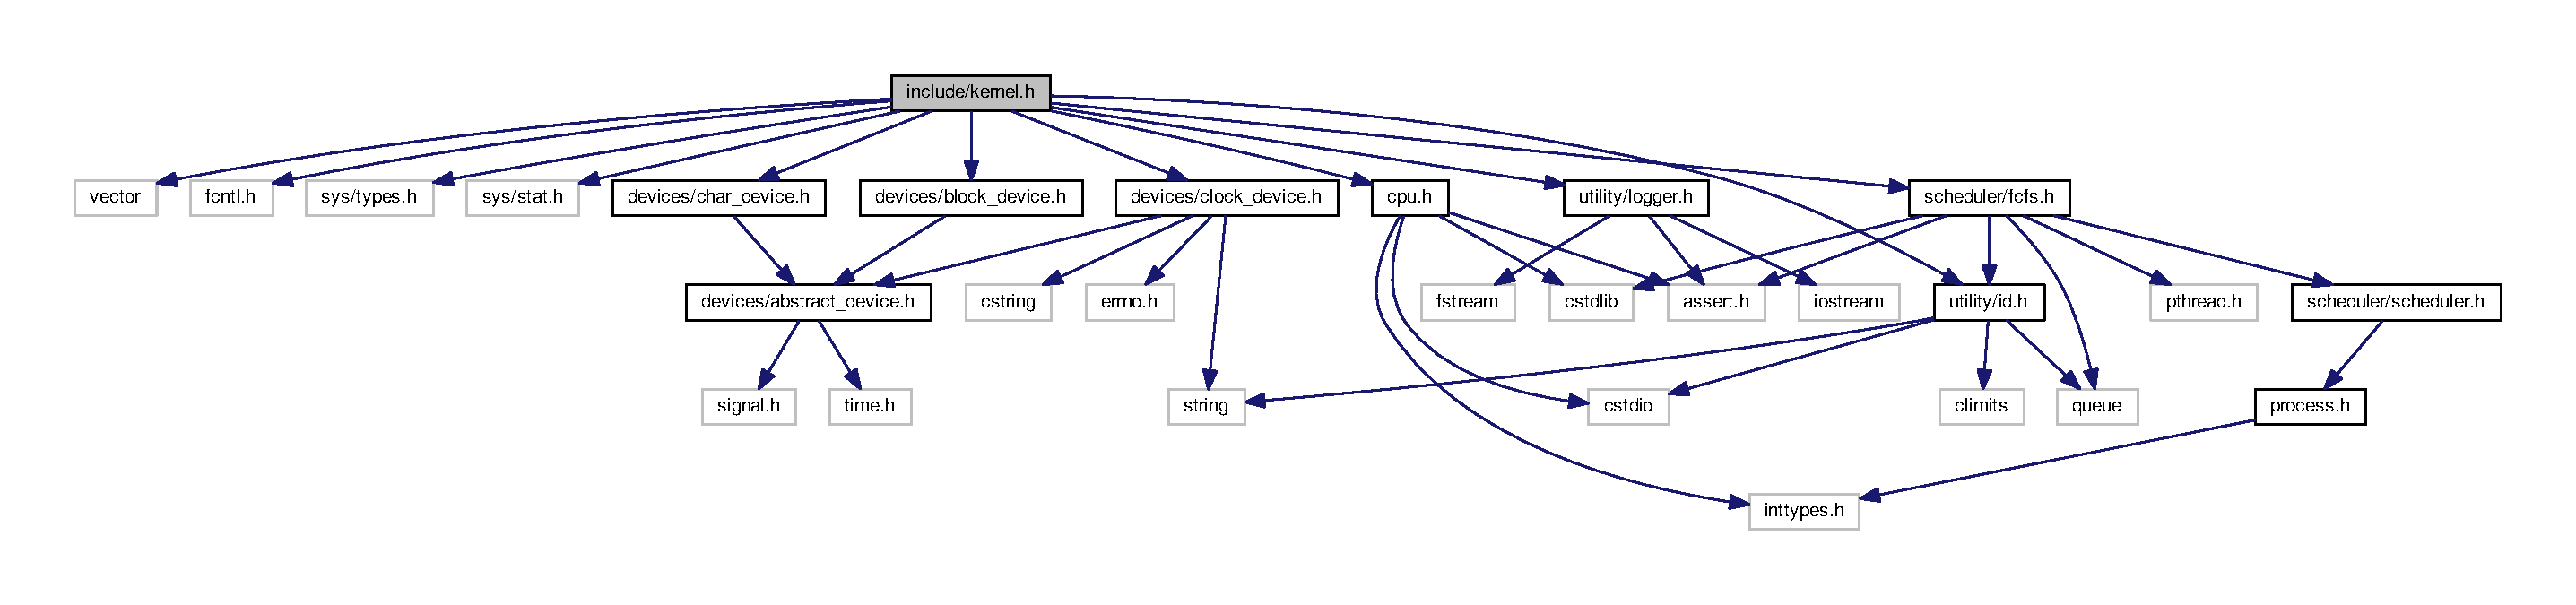
\includegraphics[width=350pt]{d4/d0f/kernel_8h__incl}
\end{center}
\end{figure}
\-This graph shows which files directly or indirectly include this file\-:\nopagebreak
\begin{figure}[H]
\begin{center}
\leavevmode
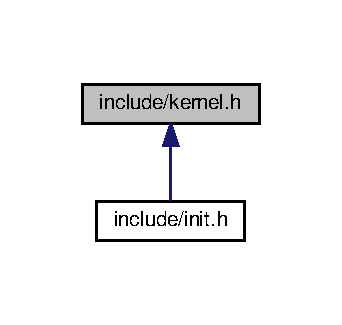
\includegraphics[width=164pt]{de/df8/kernel_8h__dep__incl}
\end{center}
\end{figure}
\subsection*{\-Classes}
\begin{DoxyCompactItemize}
\item 
class \hyperlink{classcKernel}{c\-Kernel}
\item 
struct \hyperlink{structkernelError}{kernel\-Error}
\begin{DoxyCompactList}\small\item\em \-Struct containing kernel crash information. \end{DoxyCompactList}\end{DoxyCompactItemize}
\subsection*{\-Defines}
\begin{DoxyCompactItemize}
\item 
\#define \hyperlink{kernel_8h_ac91bd56eef3f2b82894a058b7f136a21}{\-D\-E\-F\-A\-U\-L\-T\-\_\-\-T\-I\-M\-E\-R}~5000
\begin{DoxyCompactList}\small\item\em \-Default timer value for devices. \end{DoxyCompactList}\item 
\#define \hyperlink{kernel_8h_a0756f011ef667460d583017366823244}{\-D\-E\-F\-A\-U\-L\-T\-\_\-\-P\-R\-I\-O\-R\-I\-T\-Y}~5
\begin{DoxyCompactList}\small\item\em \-Default priority assigned to newly created processes. \end{DoxyCompactList}\end{DoxyCompactItemize}
\subsection*{\-Typedefs}
\begin{DoxyCompactItemize}
\item 
\hypertarget{kernel_8h_a87e7ee09eb9354187e1877a668567104}{typedef \hyperlink{classcFCFS}{c\-F\-C\-F\-S} {\bfseries scheduler\-Type}}\label{d0/daa/kernel_8h_a87e7ee09eb9354187e1877a668567104}

\end{DoxyCompactItemize}
\subsection*{\-Variables}
\begin{DoxyCompactItemize}
\item 
static const char \hyperlink{kernel_8h_a9bd73e11b6d2b66703cd822d0c2ecd32}{init\-Process\-Name} \mbox{[}$\,$\mbox{]} = \char`\"{}main.\-trace\char`\"{}
\begin{DoxyCompactList}\small\item\em \-Name of the first program to run on the system. \end{DoxyCompactList}\item 
\hypertarget{kernel_8h_a9137377ee1ea033ea5bc9f65f22d7b6e}{static const char {\bfseries trace\-Log\-File} \mbox{[}$\,$\mbox{]} = \char`\"{}trace.\-log\char`\"{}}\label{d0/daa/kernel_8h_a9137377ee1ea033ea5bc9f65f22d7b6e}

\end{DoxyCompactItemize}


\subsection{\-Detailed \-Description}


\subsection{\-Define \-Documentation}
\hypertarget{kernel_8h_a0756f011ef667460d583017366823244}{\index{kernel.\-h@{kernel.\-h}!\-D\-E\-F\-A\-U\-L\-T\-\_\-\-P\-R\-I\-O\-R\-I\-T\-Y@{\-D\-E\-F\-A\-U\-L\-T\-\_\-\-P\-R\-I\-O\-R\-I\-T\-Y}}
\index{\-D\-E\-F\-A\-U\-L\-T\-\_\-\-P\-R\-I\-O\-R\-I\-T\-Y@{\-D\-E\-F\-A\-U\-L\-T\-\_\-\-P\-R\-I\-O\-R\-I\-T\-Y}!kernel.h@{kernel.\-h}}
\subsubsection[{\-D\-E\-F\-A\-U\-L\-T\-\_\-\-P\-R\-I\-O\-R\-I\-T\-Y}]{\setlength{\rightskip}{0pt plus 5cm}\#define {\bf \-D\-E\-F\-A\-U\-L\-T\-\_\-\-P\-R\-I\-O\-R\-I\-T\-Y}~5}}\label{d0/daa/kernel_8h_a0756f011ef667460d583017366823244}
\-Only used if no other priority is provided. \hypertarget{kernel_8h_ac91bd56eef3f2b82894a058b7f136a21}{\index{kernel.\-h@{kernel.\-h}!\-D\-E\-F\-A\-U\-L\-T\-\_\-\-T\-I\-M\-E\-R@{\-D\-E\-F\-A\-U\-L\-T\-\_\-\-T\-I\-M\-E\-R}}
\index{\-D\-E\-F\-A\-U\-L\-T\-\_\-\-T\-I\-M\-E\-R@{\-D\-E\-F\-A\-U\-L\-T\-\_\-\-T\-I\-M\-E\-R}!kernel.h@{kernel.\-h}}
\subsubsection[{\-D\-E\-F\-A\-U\-L\-T\-\_\-\-T\-I\-M\-E\-R}]{\setlength{\rightskip}{0pt plus 5cm}\#define {\bf \-D\-E\-F\-A\-U\-L\-T\-\_\-\-T\-I\-M\-E\-R}~5000}}\label{d0/daa/kernel_8h_ac91bd56eef3f2b82894a058b7f136a21}
\-Measured in microseconds. 

\subsection{\-Variable \-Documentation}
\hypertarget{kernel_8h_a9bd73e11b6d2b66703cd822d0c2ecd32}{\index{kernel.\-h@{kernel.\-h}!init\-Process\-Name@{init\-Process\-Name}}
\index{init\-Process\-Name@{init\-Process\-Name}!kernel.h@{kernel.\-h}}
\subsubsection[{init\-Process\-Name}]{\setlength{\rightskip}{0pt plus 5cm}static const char {\bf init\-Process\-Name}\mbox{[}$\,$\mbox{]} = \char`\"{}main.\-trace\char`\"{}\hspace{0.3cm}{\ttfamily  \mbox{[}static\mbox{]}}}}\label{d0/daa/kernel_8h_a9bd73e11b6d2b66703cd822d0c2ecd32}
\-When the kernel object is created, this program is loaded. \-It is run once \hyperlink{classcKernel_a0ce9a2721bb1ea4d7f999198634f702d}{c\-Kernel\-::boot} is called. 
\hypertarget{process_8h}{\section{include/process.h \-File \-Reference}
\label{da/d42/process_8h}\index{include/process.\-h@{include/process.\-h}}
}
{\ttfamily \#include $<$inttypes.\-h$>$}\*
\-Include dependency graph for process.\-h\-:\nopagebreak
\begin{figure}[H]
\begin{center}
\leavevmode
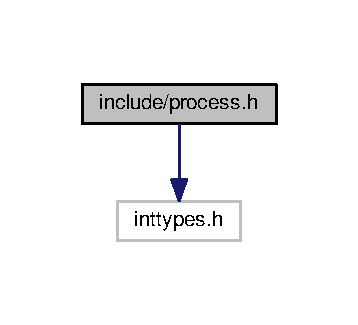
\includegraphics[width=172pt]{d5/dab/process_8h__incl}
\end{center}
\end{figure}
\-This graph shows which files directly or indirectly include this file\-:\nopagebreak
\begin{figure}[H]
\begin{center}
\leavevmode
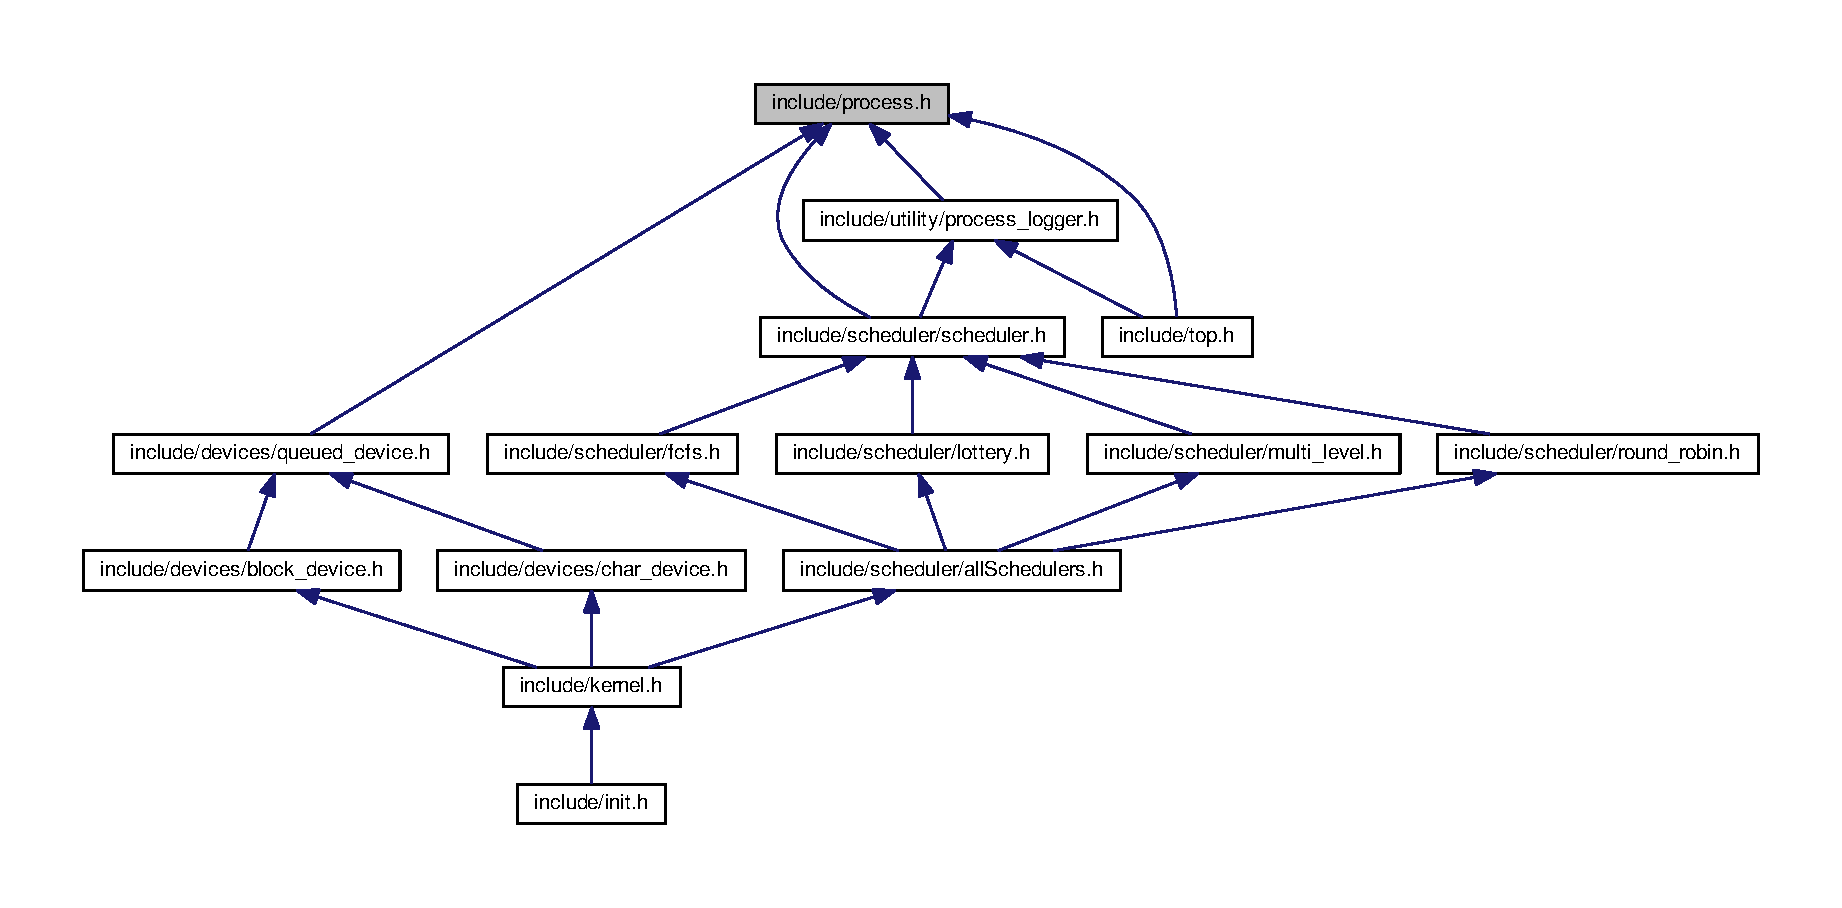
\includegraphics[width=345pt]{d1/d54/process_8h__dep__incl}
\end{center}
\end{figure}
\subsection*{\-Classes}
\begin{DoxyCompactItemize}
\item 
struct \hyperlink{structProcessInfo}{\-Process\-Info}
\begin{DoxyCompactList}\small\item\em \-Structure for containing process state and data. \end{DoxyCompactList}\end{DoxyCompactItemize}
\subsection*{\-Typedefs}
\begin{DoxyCompactItemize}
\item 
\hypertarget{process_8h_a1c804f1220f3edf8f809fa0ccfb7643f}{typedef unsigned int {\bfseries pid\-Type}}\label{da/d42/process_8h_a1c804f1220f3edf8f809fa0ccfb7643f}

\end{DoxyCompactItemize}
\subsection*{\-Enumerations}
\begin{DoxyCompactItemize}
\item 
enum \hyperlink{process_8h_a2c72cb00af5be695c1f898162350821f}{e\-Proc\-State} \{ \hyperlink{process_8h_a2c72cb00af5be695c1f898162350821fa3d4001ca586c857718be397374082d76}{ready}, 
\hyperlink{process_8h_a2c72cb00af5be695c1f898162350821faf9ccc71a0c4e71cc139d2c885154b243}{running}, 
\hyperlink{process_8h_a2c72cb00af5be695c1f898162350821fa035732e2026cb263f1bd9eee6ca6ae01}{blocked}, 
\hyperlink{process_8h_a2c72cb00af5be695c1f898162350821fa21b6f86c6d8b11d4a9c163130f55c5dd}{terminated}
 \}
\begin{DoxyCompactList}\small\item\em \-Enumeration for process states. \end{DoxyCompactList}\end{DoxyCompactItemize}


\subsection{\-Detailed \-Description}


\subsection{\-Enumeration \-Type \-Documentation}
\hypertarget{process_8h_a2c72cb00af5be695c1f898162350821f}{\index{process.\-h@{process.\-h}!e\-Proc\-State@{e\-Proc\-State}}
\index{e\-Proc\-State@{e\-Proc\-State}!process.h@{process.\-h}}
\subsubsection[{e\-Proc\-State}]{\setlength{\rightskip}{0pt plus 5cm}enum {\bf e\-Proc\-State}}}\label{da/d42/process_8h_a2c72cb00af5be695c1f898162350821f}
\-Each values defines a current state and possible transitions. \begin{Desc}
\item[\-Enumerator\-: ]\par
\begin{description}
\index{ready@{ready}!process.\-h@{process.\-h}}\index{process.\-h@{process.\-h}!ready@{ready}}\item[{\em 
\hypertarget{process_8h_a2c72cb00af5be695c1f898162350821fa3d4001ca586c857718be397374082d76}{ready}\label{da/d42/process_8h_a2c72cb00af5be695c1f898162350821fa3d4001ca586c857718be397374082d76}
}]\-Process is ready to be run. \-Invariant \-State\-:\par
 \begin{DoxyItemize}
\item \-Kernel has initialized it at some point \item \-Process should be preparred to run\end{DoxyItemize}
\-Potential \-Transitions\-: \begin{DoxyItemize}
\item \hyperlink{process_8h_a2c72cb00af5be695c1f898162350821faf9ccc71a0c4e71cc139d2c885154b243}{running} -\/ \-Scheduler picks it to run next \end{DoxyItemize}
\index{running@{running}!process.\-h@{process.\-h}}\index{process.\-h@{process.\-h}!running@{running}}\item[{\em 
\hypertarget{process_8h_a2c72cb00af5be695c1f898162350821faf9ccc71a0c4e71cc139d2c885154b243}{running}\label{da/d42/process_8h_a2c72cb00af5be695c1f898162350821faf9ccc71a0c4e71cc139d2c885154b243}
}]\-Process is currently running. \-Invariant \-State\-: \begin{DoxyItemize}
\item \-Process is on the cpu\end{DoxyItemize}
\-Potential \-Transitions\-: \begin{DoxyItemize}
\item \hyperlink{process_8h_a2c72cb00af5be695c1f898162350821fa035732e2026cb263f1bd9eee6ca6ae01}{blocked} -\/ \-Makes blocking system call \item \hyperlink{process_8h_a2c72cb00af5be695c1f898162350821fa21b6f86c6d8b11d4a9c163130f55c5dd}{terminated} -\/ \-Causes exception in cpu or finished normally \end{DoxyItemize}
\index{blocked@{blocked}!process.\-h@{process.\-h}}\index{process.\-h@{process.\-h}!blocked@{blocked}}\item[{\em 
\hypertarget{process_8h_a2c72cb00af5be695c1f898162350821fa035732e2026cb263f1bd9eee6ca6ae01}{blocked}\label{da/d42/process_8h_a2c72cb00af5be695c1f898162350821fa035732e2026cb263f1bd9eee6ca6ae01}
}]\-Process is blocked and cannot run. \-Invariant \-State\-: \begin{DoxyItemize}
\item \-Process is blocked (for now it can only block on \-I/\-O)\end{DoxyItemize}
\-Potential \-Transitions\-: \begin{DoxyItemize}
\item \hyperlink{process_8h_a2c72cb00af5be695c1f898162350821fa3d4001ca586c857718be397374082d76}{ready} -\/ \-Kernel notifies scheduler that \-I/\-O has finished \end{DoxyItemize}
\index{terminated@{terminated}!process.\-h@{process.\-h}}\index{process.\-h@{process.\-h}!terminated@{terminated}}\item[{\em 
\hypertarget{process_8h_a2c72cb00af5be695c1f898162350821fa21b6f86c6d8b11d4a9c163130f55c5dd}{terminated}\label{da/d42/process_8h_a2c72cb00af5be695c1f898162350821fa21b6f86c6d8b11d4a9c163130f55c5dd}
}]\-Process has been terminated. \-It will be cleaned up soon.

\-Invariant \-State\-: \begin{DoxyItemize}
\item \-Process either caused cpu exception or finished \item \-Process can no longer run\end{DoxyItemize}
\-Potential \-Transitions\-: \begin{DoxyItemize}
\item \-None \end{DoxyItemize}
\end{description}
\end{Desc}


\printindex
\end{document}
